\documentclass[11pt]{article}
\usepackage[T1]{fontenc}
\usepackage{lmodern}
\usepackage[margin=1in]{geometry}
\usepackage{amsmath,amssymb,amsthm,mathtools,bm}
\usepackage{microtype,graphicx,booktabs,longtable,array,enumitem,xcolor,xurl}
\usepackage[colorlinks=true,linkcolor=blue!45!black,citecolor=blue!45!black,urlcolor=blue!55!black]{hyperref}
\usepackage{bookmark}
\usepackage{fancyhdr}
\pagestyle{fancy}\fancyhf{}
\fancyhead[L]{\small A convolution calculus for Stieltjes functions}
\fancyhead[R]{\small ProveIt continuation}
\fancyfoot[C]{\thepage}
\setlength{\headheight}{14pt}
\emergencystretch=3em
\numberwithin{equation}{section}
\newtheorem{theorem}{Theorem}[section]
\newtheorem{proposition}[theorem]{Proposition}
\newtheorem{lemma}[theorem]{Lemma}
\newtheorem{corollary}[theorem]{Corollary}
\theoremstyle{definition}\newtheorem{definition}[theorem]{Definition}
\theoremstyle{remark}\newtheorem{remark}[theorem]{Remark}
\newtheorem{example}[theorem]{Example}
\DeclareMathOperator{\Li}{Li}
\DeclareMathOperator{\FP}{FP}
\DeclareMathOperator{\Res}{Res}
\DeclareMathOperator{\Rea}{Re}
\DeclareMathOperator{\Ima}{Im}
\DeclareMathOperator{\supp}{supp}
\newcommand{\dd}{\,\mathrm d}
\newcommand{\iu}{\mathrm i}
\newcommand{\R}{\mathbb R}\newcommand{\C}{\mathbb C}
\newcommand{\N}{\mathbb N}\newcommand{\Z}{\mathbb Z}
\newcommand{\Q}{\mathbb Q}\newcommand{\T}{\mathbb T}
\newcommand{\g}[1]{\gamma_{#1}}
\newcommand{\qn}[1]{\mathsf Q_{#1}}
\newcommand{\id}{\mathsf I}
\newcommand{\calG}{\mathcal G}
\newcommand{\calH}{\mathcal H}
\newcommand{\calK}{\mathcal K}
\newcommand{\calR}{\mathcal R}
\newcommand{\coef}[2]{[#1]#2}
\newcommand{\fracpart}[1]{\{#1\}}
\newcommand{\sourcepath}[1]{\texttt{\small\nolinkurl{#1}}}
\title{A Convolution Calculus for Stieltjes Functions\\[5pt]
\large Finite parts, polylogarithm jets, polygamma corrections,\\
and sharp log-Gamma correlations}
\author{Research continuation for Vladimir Reshetnikov's ProveIt project\\
\small Prepared with OpenAI assistance}
\date{10 October 2026}
\hypersetup{pdftitle={A Convolution Calculus for Stieltjes Functions},
pdfauthor={ProveIt research continuation with OpenAI assistance}}
\begin{document}
\maketitle
\begin{abstract}
We develop a bilinear extension of the Hurwitz-jet calculus in the ProveIt
polylogarithm manuscript. A classical periodic Hurwitz convolution and its
oppositely oriented correlation are continued to the pole at order one.
Explicit subtraction of the two spatial endpoint singularities gives
Hadamard finite-part integrals of arbitrary generalized Stieltjes functions.
Both orientations reduce to finite linear combinations of Stieltjes
functions at the shift and its complement, with universal coefficients in
ordinary zeta values. In particular, for $0<a<1$,
\[
\begin{aligned}
 \FP\!\int_0^1\psi(x)\psi(\{a-x\})\dd x
 &=2\gamma_1(a)+\zeta(2),\\
 \FP\!\int_0^1\psi(x)\psi(\{x+a\})\dd x
 &=\gamma_1(a)+\gamma_1(1-a)-2\zeta(2).
\end{aligned}
\]
The periodic finite-part distributions form a polynomial convolution
algebra generated by the digamma distribution. Bell polynomials describe
all its elements and retain the Dirac terms required at coincident shifts.
We determine the correction between differentiation and spatial finite
parts, obtaining an every-order digamma--polygamma integral. Ordinary
log-Gamma correlations provide a second realization of the same calculus;
we prove strict convexity, the unique half-period minimum, and an exact
convergent expansion with a sharp logarithmic cusp. A complementary moment
theorem gives strict Hankel inequalities for the Stieltjes derivative
tower. Two precisely scoped manuscript corrections and reproducible
symbolic and numerical checks accompany the proofs. Classical ingredients
and a rediscovered Dilcher series are explicitly attributed; no claim of
historical priority or resolution of the manuscript's remaining Gaussian
conjectures is made.
\end{abstract}
\clearpage
\tableofcontents
\clearpage

\section{Scope, source audit, and mathematical contribution}
\label{sec:scope}

The reference snapshot is the ProveIt commit
\begin{center}\small\texttt{570b0567f311cf1890865065896be2665f469e4f}.\end{center}
We inspected the current manuscript, its editorial ledger, and the incoming
archive register, with detailed attention to the integration,
differentiation, conductor, and distribution chapters \cite{ProveIt}.
The manuscript already proves every-index Stieltjes antiderivative and
parameter-derivative formulas, as well as substantial rational-grid and
Dirichlet-character reductions. Repeating those identities would add
little. The present development studies products at two spatial arguments,
their singular limits, and the algebra those limits create.

The main statements proved here are the finite-part coefficient theorem
(Theorem~\ref{thm:fp}), its two triangular reductions
(Theorem~\ref{thm:triangular}), the convolution algebra
(Theorem~\ref{thm:algebra}), the derivative correction
(Theorem~\ref{thm:derivative}), and the log-Gamma correlation theorem
(Theorem~\ref{thm:cusp}). Each is supplied with an analytic proof. Finite
symbolic calculations verify the displayed coefficient tables, while
independent real quadrature checks the normalization and signs.

\subsection{Prior results and the limits of the novelty claim}

Hurwitz's Fourier expansion, Lerch's gamma identity, the Hurwitz
parameter derivative, and the local polylogarithm expansion are classical
\cite{DLMFHurwitz,DLMFPolylog}. Espinosa and Moll evaluated unshifted and
reflected Hurwitz products and used them for log-Gamma integrals
\cite[Theorem 3.1 and Section 6]{EspinosaMoll}. Sun's normalized periodic
Hurwitz convolution is stated in the primary preprint
\cite[Remark 3.2]{Sun}; the published formula is also restated in
\cite[Theorem 1.6]{ZhuHuKim}. We give a short Fourier proof and the complex
parameter domain needed here. These convolution identities are therefore
building blocks, not new discoveries.

The additions relative to the audited manuscript are the explicit
separated-singularity finite-part calculus, its every-index triangular
reductions, the contact terms and derivative correction, and the resulting
sharp shifted-correlation structure. Spectral and distributional treatments
of polylogarithms are also established subjects \cite{GaySebbar}; the
proofs below do not establish a first-in-the-literature claim for every
specialization. The positive series for $\gamma_1$ in
Section~\ref{sec:dilcher} is equivalent to a formula attributed to Dilcher
in Brede's dissertation \cite{Dilcher,Brede}; it is retained as a consistency
check and an application of the correlation geometry.

No audited source states the present convolution problem as an explicit
conjecture. Thus this is a proved continuation rather than a claimed
resolution of a named existing conjecture. In particular, $S_6$ and the
distinct new frozen $S_8$ candidate at \texttt{s8new:conj:S8} retain their
conjectural status. An earlier, different $S_8$ vector was already
rigorously rejected at \texttt{research:prop:S8-rejected}; it is not an
open conjecture. The already integrated $S_4$ proof is not reproved here.

\section{Conventions and analytic preparation}
\label{sec:conventions}

For $x>0$ we use
\begin{equation}\label{eq:laurent}
 \zeta(1+u,x)=\frac1u+
 \sum_{n=0}^{\infty}\frac{(-1)^n}{n!}\gamma_n(x)u^n,
 \qquad \gamma_0(x)=-\psi(x).
\end{equation}
The prime on $\zeta(s,x)$ denotes differentiation in $s$; a superscript
$\gamma_n^{(k)}(x)$ or $\psi^{(k)}(x)$ denotes differentiation in $x$.
Set
\begin{equation}\label{eq:H}
 H(u,x)=\zeta(1+u,x)-\frac1u.
\end{equation}
It is holomorphic in $u$ at zero for fixed $x>0$. The shift identity gives
\begin{equation}\label{eq:localH}
 H(u,x)=x^{-1-u}+H(u,1+x),\qquad
 \gamma_n(x)=\frac{\log^n x}{x}+\gamma_n(1+x).
\end{equation}
These formulas fix every endpoint subtraction used below.

Let $\T=\R/\Z$ and write $\{x\}$ for the fractional part. Values at the
isolated integers do not affect an ordinary integral; at those points a
finite-part or distributional prescription will always be stated. For
$0<a<1$, put $b=1-a$ and define the two orientations
\begin{align}
 C^-_{f,g}(a)&=\int_0^1 f(x)g(\{a-x\})\dd x,
       \label{eq:minusdef}\\
 C^+_{f,g}(a)&=\int_0^1 f(x)g(\{x+a\})\dd x.
       \label{eq:plusdef}
\end{align}
The minus sign denotes ordinary periodic convolution. The plus sign
denotes correlation without complex conjugation. This distinction matters
when the two functions differ.

For $k\ne0$ we take
\begin{equation}\label{eq:logbranch}
 \log(2\pi\iu k)=\log(2\pi|k|)
                   +\frac{\pi\iu}{2}\operatorname{sgn}k.
\end{equation}
Polylogarithms on the unit circle away from $1$ are their standard
analytic continuations from the unit disk. They are entire in the order
there. The identities will initially be proved where their Fourier series
converge absolutely, then continued with the spatial singularities kept
separate.

\begin{lemma}[Mean and Fourier coefficients]\label{lem:fourier}
For $\Rea s<1$, the function $x\mapsto\zeta(s,x)$ is integrable on $(0,1)$
and has mean zero. For $\Rea s<0$ its absolutely convergent Fourier series is
\begin{equation}\label{eq:fourier}
 \zeta(s,x)=\Gamma(1-s)\sum_{k\ne0}
                     (2\pi\iu k)^{s-1}e^{2\pi\iu kx}.
\end{equation}
\end{lemma}
\begin{proof}
The shift identity isolates $x^{-s}$ and a function smooth at zero.
Hence integrability follows for $\Rea s<1$. Integrate
$\partial_x\zeta(s-1,x)=(1-s)\zeta(s,x)$ and use
$x^{1-s}\to0$ to obtain zero mean. Equation~\eqref{eq:fourier} is
Hurwitz's Fourier expansion \cite[25.11.9]{DLMFHurwitz}; its two half-series
have terms of magnitude $O(|k|^{\Rea s-1})$, proving absolute convergence
in the stated half-plane.
\end{proof}

\section{The two Hurwitz convolution formulas}
\label{sec:hurwitz}

\begin{theorem}[Classical convolution and shifted correlation]
\label{thm:classical}
Let $0<a<1$, $\Rea s<1$, and $\Rea t<1$. Then
\begin{equation}\label{eq:hurwitzminus}
 \calK_-(s,t;a):=C^-_{\zeta(s,\cdot),\zeta(t,\cdot)}(a)
 =\frac{\Gamma(1-s)\Gamma(1-t)}{\Gamma(2-s-t)}
                         \zeta(s+t-1,a).
\end{equation}
For $\theta=2\pi a$ the other orientation is
\begin{align}\label{eq:hurwitzplus}
 \calK_+(s,t;a)
 ={}&\Gamma(1-s)\Gamma(1-t)(2\pi)^{s+t-2}\notag\\
 &\quad\times\left[
 e^{\pi\iu(s-t)/2}\Li_{2-s-t}(e^{-\iu\theta})
 +e^{-\pi\iu(s-t)/2}\Li_{2-s-t}(e^{\iu\theta})\right].
\end{align}
Both equalities are jointly holomorphic in this domain. Every fixed finite
number of spectral derivatives can be passed through the integrals.
\end{theorem}
\begin{proof}
First suppose $\Rea s,\Rea t<0$. For the minus orientation, Fourier
orthogonality selects equal frequencies, so the coefficient at $k\ne0$ is
\[
 \Gamma(1-s)\Gamma(1-t)(2\pi\iu k)^{s+t-2}.
\]
Comparing with \eqref{eq:fourier} at order $s+t-1$ proves
\eqref{eq:hurwitzminus}. For the plus orientation, orthogonality selects
opposite frequencies, giving
\[
 \Gamma(1-s)\Gamma(1-t)
 \sum_{k\ne0}(2\pi\iu k)^{s-1}
             (-2\pi\iu k)^{t-1}e^{-2\pi\iu ka}.
\]
Separate positive and negative $k$ and use \eqref{eq:logbranch}; the result
is exactly \eqref{eq:hurwitzplus}.

In the minus integral the singularities occur at $x=0^+$ and $x=a^-$.
In the plus integral they occur at $x=0^+$ and $x=b^+$. They are separated
for fixed $0<a<1$. On a compact subset of $\Rea s,\Rea t<1$, local
majorants have the form $x^{-\sigma}(1+|\log x|^r)$ with $\sigma<1$.
They justify joint holomorphy and spectral differentiation under the
integral. The right sides are holomorphic in the same domain; for
\eqref{eq:hurwitzminus}, $\Rea(2-s-t)>0$ and $s+t-1\ne1$.
The identity theorem, first in one variable and then the other, extends
the formulas throughout this connected product of half-planes.
\end{proof}

The orientation reversal cannot be omitted: at $s=t=0$ the first formula
is $\zeta(-1,a)$, whereas the second is $-\zeta(-1,a)$. At $a=0$ the
plus integral has coincident singularities and requires an additional
integrability condition. We keep $0<a<1$ in all finite-part formulas.

\section{Hadamard finite parts at order one}
\label{sec:finiteparts}

\begin{definition}[The two spatial finite parts]\label{def:fp}
For $n,m\ge0$ and $0<a<1$, define
\begin{align}\label{eq:fpminus}
 F^-_{n,m}(a)=\lim_{\epsilon,\eta\downarrow0}
 \bigg\{&\int_{\epsilon}^{a-\eta}
 \gamma_n(x)\gamma_m(a-x)\dd x
 +\int_a^1\gamma_n(x)\gamma_m(1+a-x)\dd x\notag\\
 &+\frac{\gamma_m(a)}{n+1}\log^{n+1}\epsilon
  +\frac{\gamma_n(a)}{m+1}\log^{m+1}\eta\bigg\}.
\end{align}
With $b=1-a$, define
\begin{align}\label{eq:fpplus}
 F^+_{n,m}(a)=\lim_{\epsilon,\eta\downarrow0}
 \bigg\{&\int_{\epsilon}^{b}\gamma_n(x)\gamma_m(x+a)\dd x
 +\int_{b+\eta}^{1}\gamma_n(x)\gamma_m(x-b)\dd x\notag\\
 &+\frac{\gamma_m(a)}{n+1}\log^{n+1}\epsilon
  +\frac{\gamma_n(b)}{m+1}\log^{m+1}\eta\bigg\}.
\end{align}
The two cutoffs tend to zero independently. The powers of their logarithms
use the actual coordinates displayed here, fixing the normalization.
\end{definition}

The limits exist: after the leading singular term is subtracted, each
remaining local integrand is $O(1+|\log x|^{\max(n,m)})$. Thus these
definitions can also be evaluated by ordinary convergent integrals.

Set $w=u+v$ and introduce
\begin{equation}\label{eq:E}
 E(u,v)=\frac{\Gamma(1-u)\Gamma(1-v)}{\Gamma(1-w)}.
\end{equation}
The two holomorphic numerator germs are
\begin{equation}\label{eq:Bminus}
 B_-(u,v;a)=-E(u,v)\bigl(1+wH(w,a)\bigr),
\end{equation}
and
\begin{align}\label{eq:Bplus}
 B_+(u,v;a)={}&\Gamma(1-u)\Gamma(1-v)(2\pi)^w\notag\\
 &\times\left[e^{\pi\iu(u-v)/2}\Li_{-w}(e^{-2\pi\iu a})
              +e^{-\pi\iu(u-v)/2}\Li_{-w}(e^{2\pi\iu a})\right].
\end{align}
They satisfy $B_\pm(0,0;a)=-1$. Define the mixed divided difference
\begin{equation}\label{eq:Rgerm}
 \calR_\pm(u,v;a)=
 \frac{B_\pm(u,v;a)-B_\pm(u,0;a)-B_\pm(0,v;a)+B_\pm(0,0;a)}{uv}.
\end{equation}
It is holomorphic even when $u=0$ or $v=0$.

\begin{theorem}[Every-index finite-part coefficient formula]\label{thm:fp}
For all $n,m\ge0$ and $0<a<1$,
\begin{equation}\label{eq:fpcoefficient}
 F^\pm_{n,m}(a)=(-1)^{n+m}n!m!\,[u^nv^m]\calR_\pm(u,v;a)
 =(-1)^{n+m}n!m!\,[u^{n+1}v^{m+1}]B_\pm(u,v;a).
\end{equation}
Thus \eqref{eq:Bplus} is an explicit integral identity involving
polylogarithm order derivatives at zero, gamma derivatives at one, and
arbitrary Stieltjes functions.
\end{theorem}
\begin{proof}
For $\Rea u,\Rea v<0$ near zero, the product of the two functions $H$ is
integrable. Since the mean of each Hurwitz zeta is zero,
\begin{equation}\label{eq:HH}
 C^\pm_{H(u,\cdot),H(v,\cdot)}(a)
 =\calK_\pm(1+u,1+v;a)+\frac1{uv}
 =\frac{B_\pm(u,v;a)+1}{uv}.
\end{equation}
The sign of the final $1/(uv)$ follows by expanding the two pole
subtractions and using the zero means; it is essential.

Near the first singularity, \eqref{eq:localH} shows that the integrand
equals $x^{-1-u}H(v,a)$ plus a locally integrable holomorphic remainder.
Integrating this term meromorphically gives residue $-H(v,a)$ at $u=0$.
At the second singularity the residue at $v=0$ is $-H(u,a)$ in the minus
orientation and $-H(u,b)$ in the plus orientation. No other nearby poles
occur, since after these terms are subtracted the remainders are bounded
by $x^{-r}$ with $r<1$ on a sufficiently small bidisk.

Consequently the holomorphic regularizations are respectively
\begin{align*}
 \frac{B_-+1}{uv}+\frac{H(v,a)}u+\frac{H(u,a)}v,\qquad
 \frac{B_++1}{uv}+\frac{H(v,a)}u+\frac{H(u,b)}v.
\end{align*}
Equivalently, the boundary identities are
\begin{align}\label{eq:boundaries}
 B_-(u,0;a)&=-1-uH(u,a),& B_-(0,v;a)&=-1-vH(v,a),\notag\\
 B_+(u,0;a)&=-1-uH(u,b),& B_+(0,v;a)&=-1-vH(v,a).
\end{align}
These yield exactly \eqref{eq:Rgerm}.

To identify the coefficients with the specified spatial finite parts,
use
\[
 \int_\epsilon^c x^{-1-u}\dd x
 =\frac{\epsilon^{-u}-c^{-u}}u.
\]
The coefficient of $(-u)^n/n!$ in the subtracted endpoint contribution
is $\log^{n+1}\epsilon/(n+1)$, with exactly the signs in
\eqref{eq:fpminus}--\eqref{eq:fpplus}. The regular remainders and their
spectral derivatives are dominated by integrable logarithmic powers.
Coefficient extraction and the two cutoff limits therefore commute.
This proves both identities in \eqref{eq:fpcoefficient}.
\end{proof}

\section{Triangular reduction to Stieltjes functions}
\label{sec:triangular}

The polylogarithm representation is not the end of the reduction. Introduce
\begin{equation}\label{eq:Fgamma}
 T(u,v)=\frac{\Gamma(1-u)\Gamma(1+u+v)}{\Gamma(1+v)},\qquad
 U(u,v)=T(v,u),\qquad
 V(u,v)=\frac{vT(u,v)+uU(u,v)}{u+v}.
\end{equation}
The quotient defining $V$ is holomorphic: on $v=-u$ both $T$ and $U$
equal $1$, so its numerator vanishes. A holomorphic function vanishing on
that hyperplane is divisible by $u+v$.

\begin{proposition}[Gamma-only numerator]\label{prop:gammaonly}
For $b=1-a$,
\begin{equation}\label{eq:Bplusgamma}
 B_+(u,v;a)=-V(u,v)-vT(u,v)H(u+v,a)-uU(u,v)H(u+v,b).
\end{equation}
\end{proposition}
\begin{proof}
Apply the two Hurwitz Fourier equations at arguments $a,b$ and order
$1+w$ to the two polylogarithms in \eqref{eq:Bplus}. Solving this
two-by-two linear system first where $\sin\pi w\ne0$ gives
\[
 B_+=-E(u,v)\frac{w}{\sin\pi w}
 \left[\sin\pi v\,\zeta(1+w,a)+\sin\pi u\,\zeta(1+w,b)\right].
\]
Euler's reflection identity gives
\[
 E(u,v)\frac{\sin\pi v}{\sin\pi w}=\frac v w T(u,v),\qquad
 E(u,v)\frac{\sin\pi u}{\sin\pi w}=\frac u w U(u,v).
\]
Substitute $\zeta(1+w,x)=1/w+H(w,x)$ and cancel. The resulting
\eqref{eq:Bplusgamma} extends across $w=0$ by holomorphy.
\end{proof}

The relevant gamma quotients have the convergent logarithmic expansions
\begin{align}
 \log E(u,v)&=\sum_{r\ge2}\frac{\zeta(r)}r
                 \bigl(u^r+v^r-(u+v)^r\bigr),\label{eq:logE}\\
 \log T(u,v)&=\sum_{r\ge2}\frac{\zeta(r)}r
                 \bigl(u^r+(-1)^r((u+v)^r-v^r)\bigr).
                 \label{eq:logT}
\end{align}
They hold when $|u|,|v|,|u+v|<1$. The Euler constant cancels completely.

\begin{theorem}[Finite triangular reductions]\label{thm:triangular}
For $n,m\ge0$, $F^-_{n,m}(a)$ is a finite linear combination of $1$ and
$\gamma_j(a)$, $0\le j\le n+m+1$. Its leading term is
\begin{equation}\label{eq:leadminus}
 \frac{n+m+2}{(n+1)(m+1)}\gamma_{n+m+1}(a).
\end{equation}
Similarly, $F^+_{n,m}(a)$ is a finite linear combination of $1$,
$\gamma_j(a)$, and $\gamma_j(b)$, with leading terms
\begin{equation}\label{eq:leadplus}
 \frac{\gamma_{n+m+1}(a)}{n+1}
 +\frac{\gamma_{n+m+1}(b)}{m+1}.
\end{equation}
All coefficients belong to $\Q[\zeta(2),\ldots,\zeta(n+m+2)]$.
The terms with index $n+m$ are absent in both orientations. The formulas
are constructive through \eqref{eq:Bminus}, \eqref{eq:Bplusgamma},
\eqref{eq:logE}, and \eqref{eq:logT}.
\end{theorem}
\begin{proof}
The target coefficient has total degree $n+m+2$. Only finitely many
terms of each displayed convergent germ can contribute. The highest
Stieltjes term in $B_-$ comes from
$-(-1)^{n+m+1}\gamma_{n+m+1}(a)(u+v)^{n+m+2}/(n+m+1)!$.
Multiply its coefficient by $(-1)^{n+m}n!m!$ to obtain
\eqref{eq:leadminus}. In \eqref{eq:Bplusgamma}, the factors $v$ and $u$
give the two binomial coefficients leading to \eqref{eq:leadplus}.
There are no degree-one terms in $E,T,U$, which proves the missing-index
assertion. Equations~\eqref{eq:logE}--\eqref{eq:logT} prove the coefficient
ring statement without any numerical relation search.
\end{proof}

\subsection{Low-order identities}

Here and below $\zeta_r=\zeta(r)$; in the following formulas all unmarked
$\gamma_j$ on the right are evaluated at $a$:
\begin{align}
 F^-_{0,0}&=2\gamma_1+\zeta_2,\label{eq:F00minus}\\
 F^-_{1,0}&=\frac32\gamma_2-\zeta_2\gamma_0-\zeta_3,\label{eq:F10minus}\\
 F^-_{1,1}&=\gamma_3-2\zeta_2\gamma_1+2\zeta_3\gamma_0
                         +\frac14\zeta_4,\label{eq:F11minus}\\
 F^-_{2,0}&=\frac43\gamma_3-2\zeta_2\gamma_1+2\zeta_3\gamma_0
                         +2\zeta_4.\label{eq:F20minus}
\end{align}
In \eqref{eq:F11minus} we used $\zeta_2^2=\tfrac52\zeta_4$.
The reflected identities are symmetric in $n,m$. For the other orientation,
\begin{align}
 F^+_{0,0}(a)&=\gamma_1(a)+\gamma_1(b)-2\zeta_2,
       \label{eq:F00plus}\\
 F^+_{1,0}(a)&=\frac12\gamma_2(a)+\gamma_2(b)
       +\zeta_2\bigl(\gamma_0(a)+\gamma_0(b)\bigr)-\zeta_3,
       \label{eq:F10plus}\\
 F^+_{1,1}(a)&=\frac{\gamma_3(a)+\gamma_3(b)}2
       +2\zeta_2\bigl(\gamma_1(a)+\gamma_1(b)\bigr)\notag\\
       &\qquad+\zeta_3\bigl(\gamma_0(a)+\gamma_0(b)\bigr)
                     -\frac72\zeta_4.\label{eq:F11plus}
\end{align}
One has $F^+_{n,m}(a)=F^+_{m,n}(b)$, rather than symmetry at a fixed $a$.

\begin{corollary}[One digamma factor, every Stieltjes index]
\label{cor:onedigamma}
For $n\ge0$,
\begin{align}\label{eq:onedigamma}
 F^-_{n,0}(a)={}&\frac{n+2}{n+1}\gamma_{n+1}(a)
 +\sum_{j=1}^{n}(-1)^j\frac{n!}{(n-j)!}
                 \zeta(j+1)\gamma_{n-j}(a)\notag\\
 &+(-1)^n n!\zeta(n+2).
\end{align}
\end{corollary}
\begin{proof}
Differentiate \eqref{eq:logE} in $v$ at zero to get
$E(u,v)=1-v\sum_{j\ge1}\zeta(j+1)u^j+O(v^2)$.
Insert this in \eqref{eq:Bminus}, extract $[u^{n+1}v]$, and apply
Theorem~\ref{thm:fp}. This also independently verifies the entire first
column of the coefficient table.
\end{proof}

\subsection{A polylogarithm order-derivative identity}

Put $A=\gamma+\log(2\pi)$ and $z=e^{2\pi\iu a}$. Directly differentiating
\eqref{eq:Bplus} at $u=v=0$ yields
\begin{equation}\label{eq:Li0identity}
 2\Rea\left.\partial_s^2\Li_s(z)\right|_{s=0}
 -4A\Rea\left.\partial_s\Li_s(z)\right|_{s=0}
 =\gamma_1(a)+\gamma_1(b)+A^2-\frac{\pi^2}{12}.
\end{equation}
Indeed $\Li_0(z)+\Li_0(z^{-1})=-1$, and the phase derivatives contribute
$-\pi^2/4$ to $F^+_{0,0}$. Equation~\eqref{eq:F00plus} then gives
\eqref{eq:Li0identity}. This identity is also a useful independent
normalization check on the two-variable germ.

For example, writing $\gamma_1=\gamma_1(1)$, one obtains
\begin{align}
 F^+_{0,0}(\tfrac12)
 &=2\gamma_1-4\gamma\log2-2\log^22-\frac{\pi^2}{3},\label{eq:halfFP}\\
 F^+_{0,0}(\tfrac13)
 &=2\gamma_1-3\gamma\log3-\frac32\log^23-\frac{\pi^2}{3},\label{eq:thirdFP}\\
 F^+_{0,0}(\tfrac14)
 &=2\gamma_1-6\gamma\log2-7\log^22-\frac{\pi^2}{3}.
       \label{eq:quarterFP}
\end{align}
They follow either from Hurwitz distribution at the indicated moduli or
from the root-of-unity polylogarithms in \eqref{eq:Bplus}. No arithmetic
independence claim is involved.

\section{The periodic distribution algebra}
\label{sec:algebra}

The preceding integrals deliberately exclude the coincident shift. To
describe convolution on the whole circle, including that point, one must
retain distributions supported at zero. Let $\delta_0$ be the periodic
Dirac distribution, let $1$ denote the constant distribution, and put
\begin{equation}\label{eq:unit}
 \id=\delta_0-1.
\end{equation}
On the space of distributions with mean zero, $\id$ is the convolution
identity. It is not the identity on all periodic distributions.

For a smooth periodic test function $\phi$, define
\begin{equation}\label{eq:Qdefinition}
 \langle\qn n,\phi\rangle
 =\int_0^1\frac{\log^n x}{x}\bigl(\phi(x)-\phi(0)\bigr)\dd x
   +\int_0^1\gamma_n(1+x)\phi(x)\dd x.
\end{equation}
Thus $\qn n$ is the scale-one finite part of $\gamma_n$.
Its mean is zero: the first integral vanishes for $\phi=1$, and
$\int_1^2\zeta(1+u,x)\dd x=1/u$ implies
$\int_1^2\gamma_n(x)\dd x=0$.

Let $Z(u)$ be the meromorphic distribution obtained by continuing
$\zeta(1+u,x)$ from $\Rea u<0$. The singular monomial $x^{-1-u}$
has residue $-\delta_0$, while the regular shifted Hurwitz term has
residue $1$. Consequently
\begin{equation}\label{eq:Zdistribution}
 Z(u)=-\frac{\id}{u}+\calG(u),\qquad
 \calG(u)=\sum_{n\ge0}\frac{(-1)^n}{n!}\qn n u^n.
\end{equation}
The series is holomorphic near zero in the distribution sense. A useful
distinction is that the pointwise holomorphic function $H(u,x)$ in
\eqref{eq:H}, when continued as a distribution, still has residue
$-\delta_0$. Pointwise pole subtraction and spatial continuation do not
remove the same pole.

\begin{theorem}[A polynomial convolution algebra]\label{thm:algebra}
Let $Y_j$ be the complete exponential Bell polynomials, defined by
\[
 \exp\left(\sum_{j\ge1}x_j\frac{u^j}{j!}\right)
 =\sum_{j\ge0}Y_j(x_1,\ldots,x_j)\frac{u^j}{j!}.
\]
Interpret multiplication as periodic convolution and the scalar unit as
$\id$. Then
\begin{equation}\label{eq:Bell}
 \qn n=\frac{(-1)^{n+1}}{n+1}
 Y_{n+1}\bigl(-\qn0,\,1!\zeta(2)\id,\,2!\zeta(3)\id,
                  \ldots,n!\zeta(n+1)\id\bigr).
\end{equation}
For $n=0$ the list consists only of $-\qn0$. In particular,
\begin{align}
 \qn0*\qn0&=2\qn1-\zeta(2)\id,\label{eq:Qsquare}\\
 \qn0*\qn0*\qn0&=3\qn2-3\zeta(2)\qn0+2\zeta(3)\id.
 \label{eq:Qcube}
\end{align}
The algebra $\operatorname{span}_{\C}\{\id,\qn0,\qn1,\ldots\}$ is
isomorphic to $\C[X]$ under $X\mapsto\qn0$.
\end{theorem}
\begin{proof}
Define $P_u$ by its Fourier coefficients
\[
 \widehat P_u(k)=
 \begin{cases}(2\pi\iu k)^u,&k\ne0,\\0,&k=0.\end{cases}
\]
On compact parameter sets these coefficients have at most polynomial
growth in $k$. Pairing with the rapidly decreasing coefficients of a
smooth test function therefore proves that $P_u$ is an entire
distribution family. Fourier multiplication gives
\[
 P_0=\id,\qquad P_u*P_v=P_{u+v},\qquad
 Z(u)=-\frac{\Gamma(1-u)}u P_u.
\]
The last equality follows first from Lemma~\ref{lem:fourier}, then by
meromorphic continuation. Comparing the constant term at $u=0$ gives
\begin{equation}\label{eq:Q0fourier}
 \widehat{\qn0}(k)=-\gamma-\log(2\pi\iu k),\qquad k\ne0.
\end{equation}
The classical expansion
$\log\Gamma(1-u)=\gamma u+\sum_{j\ge2}\zeta(j)u^j/j$
now yields the distribution identity
\begin{equation}\label{eq:convolutionexp}
 u\calG(u)=\id-\exp_*\left(
 -u\qn0+\sum_{j\ge2}\frac{\zeta(j)}j u^j\id\right),\qquad |u|<1.
\end{equation}
Here the convolution exponential is justified by the Fourier family
already constructed; no convergence assertion about arbitrary
distribution exponentials is needed. Extracting coefficients proves
\eqref{eq:Bell}.

The leading term of $\qn n$ is $\qn0^{*(n+1)}/(n+1)$, so the indicated
span is precisely the algebra generated by $\qn0$ and $\id$. If a
polynomial $p$ satisfies $p(\qn0)=0$, its nonzero Fourier coefficients give
$p(-\gamma-\log(2\pi\iu k))=0$ for every positive integer $k$.
These are infinitely many distinct arguments, so $p$ is the zero
polynomial. This proves injectivity and the claimed isomorphism.
\end{proof}

This functional algebraic independence does not imply rational or
algebraic independence of any numerical special values. The proof uses
the distinct Fourier frequencies, not unproved arithmetic assertions.

\begin{proposition}[The full binary generating identity]\label{prop:global}
With $w=u+v$ and $E$ as in \eqref{eq:E},
\begin{equation}\label{eq:globalbinary}
 \calG(u)*\calG(v)=
 \frac{u\calG(u)+v\calG(v)-wE(u,v)\calG(w)
                  +(E(u,v)-1)\id}{uv}.
\end{equation}
The quotient is removable on both axes. Its restriction to $0<a<1$
is the finite-part germ $\calR_-(u,v;a)$.
\end{proposition}
\begin{proof}
Multiply
$u\calG(u)=\id-\Gamma(1-u)P_u$ and
$v\calG(v)=\id-\Gamma(1-v)P_v$ using the semigroup law for $P$.
Since $\Gamma(1-u)\Gamma(1-v)=E(u,v)\Gamma(1-w)$, expansion gives
\eqref{eq:globalbinary}. Each $\qn n$ is smooth away from zero. At a
nonzero shift the singular supports in the integral defining convolution
are disjoint. A partition of unity around the two singularities therefore
identifies its value with the separate cutoff finite parts in
Definition~\ref{def:fp}. This proves the restriction assertion.
\end{proof}

For clarity, the complete first reflected identity is
\begin{equation}\label{eq:contactminus}
 \qn0*\qn0=2\qn1+\zeta(2)\,1-\zeta(2)\delta_0.
\end{equation}
Let $\check Q(a)=Q(-a)$ denote reflection of a periodic distribution.
The corresponding complete circular identity is
\begin{equation}\label{eq:contactplus}
 \check{\qn0}*\qn0
 =\qn1+\check{\qn1}-2\zeta(2)\,1+2\zeta(2)\delta_0.
\end{equation}
For $k\ne0$, put $c_k=\gamma+\log(2\pi|k|)$. Its two sides have
Fourier coefficient $c_k^2+\pi^2/4$, as follows from
\eqref{eq:Q0fourier} and
$\widehat{\qn1}(k)=((\gamma+\log(2\pi\iu k))^2+\zeta(2))/2$.
Their zero coefficients also agree. Omitting the Dirac terms in these
global identities would contradict the zero mean; omitting them in the
interior formulas is legitimate because $a\ne0$.

\begin{proposition}[The joint algebra of both orientations]
\label{prop:jointalgebra}
Let
\[
 \mathsf X=\frac{\qn0+\check{\qn0}}2,\qquad
 \mathsf J=\frac{\check{\qn0}-\qn0}{\pi\iu}.
\]
The finite convolution algebra generated by all $\qn n$ and their
reflections is
\begin{equation}\label{eq:jointalgebra}
 \C[X,J]/(J^2-1)\ \cong\ \C[X]\times\C[X],
\end{equation}
under $X\mapsto\mathsf X$, $J\mapsto\mathsf J$, and $1\mapsto\id$.
\end{proposition}
\begin{proof}
At a nonzero frequency $k$, the Fourier coefficients are
$\widehat{\mathsf X}(k)=-\gamma-\log(2\pi|k|)$ and
$\widehat{\mathsf J}(k)=\operatorname{sgn}k$. Both means are zero;
hence $\mathsf J*\mathsf J=\id$. Conversely
$\qn0=\mathsf X-(\pi\iu/2)\mathsf J$ and
$\check{\qn0}=\mathsf X+(\pi\iu/2)\mathsf J$, and all other generators
are Bell polynomials in these two. If
$p(\mathsf X)+\mathsf J*q(\mathsf X)=0$, its positive and negative
Fourier coefficients imply that both $p+q$ and $p-q$ vanish at every
$-\gamma-\log(2\pi n)$, $n\ge1$. Thus $p=q=0$, proving that
$J^2-1$ is the full ideal of relations. Evaluation at $J=1$ and $J=-1$
gives the last isomorphism. This assertion concerns finite polynomials,
with no topological closure implicit.
\end{proof}

\section{Differentiation of finite parts and polygamma products}
\label{sec:derivatives}

Differentiating a finite-part distribution is not always the same
operation as taking the raw finite part of the pointwise derivative.
We specify the latter without an implicit choice of additive constants.
For integers $m,n\ge0$, let $T_{m,n}=\FP[x^{-m-1}\log^n x]$ mean
\begin{align}\label{eq:powerFP}
 \langle T_{m,n},\phi\rangle={}&
 \int_0^1x^{-m-1}\log^n x
 \left(\phi(x)-\sum_{j=0}^m\frac{\phi^{(j)}(0)}{j!}x^j\right)\dd x
 \notag\\
 &+\sum_{j=0}^{m-1}\frac{\phi^{(j)}(0)}{j!}
             \frac{(-1)^n n!}{(j-m)^{n+1}}.
\end{align}
The second sum is empty when $m=0$. This is exactly the constant term of
the cutoff integral at scale one after all divergent powers and
logarithms have been removed. Apply \eqref{eq:powerFP} to the singular
polynomial in the derivative of \eqref{eq:localH}, and integrate its
smooth remainder ordinarily. Denote the resulting distribution by
$P_{n,k}=\FP\gamma_n^{(k)}$; set $P_{n,0}=\qn n$.

Let $e_j$ denote an elementary symmetric polynomial and
$H_k^{(j)}=\sum_{r=1}^k r^{-j}$, with $H_k=H_k^{(1)}$.

\begin{theorem}[The derivative correction]\label{thm:derivative}
For every $n\ge0$ and $k\ge1$,
\begin{equation}\label{eq:derivativeanomaly}
 P_{n,k}=D^k\qn n+c_{n,k}\delta_0^{(k)},\qquad
 c_{n,k}=(-1)^n n!\,e_{n+1}\left(1,\frac12,\ldots,\frac1k\right).
\end{equation}
In particular, $c_{0,k}=H_k$, and $c_{n,k}=0$ when $n\ge k$.
\end{theorem}
\begin{proof}
The meromorphic continuation $X_m(u)$ of $x^{-m-1-u}$ is obtained by
subtracting the test-function Taylor polynomial in \eqref{eq:powerFP}.
Integration of its monomials gives
\[
 \langle X_m(u),\phi\rangle
 =\int_0^1x^{-m-1-u}(\phi-\operatorname{Taylor}_m\phi)\dd x
   +\sum_{j=0}^m\frac{\phi^{(j)}(0)}{j!(j-m-u)}.
\]
Using $\langle\delta_0^{(m)},\phi\rangle=(-1)^m\phi^{(m)}(0)$,
its Laurent expansion is
\begin{equation}\label{eq:Xpole}
 X_m(u)=-\frac{(-1)^m}{m!u}\delta_0^{(m)}
               +\sum_{n\ge0}\frac{(-1)^n}{n!}T_{m,n}u^n.
\end{equation}
On the half-plane $\Rea u<-k$, the derivatives through order $k-1$ of
$\zeta(1+u,x)$ match at the periodic endpoints and its $k$th derivative is
integrable. Thus ordinary integration by parts and meromorphic
continuation give
\[
 D^k Z(u)=(-1)^k(1+u)_k
                \bigl[X_k(u)+\zeta(k+1+u,1+x)\bigr].
\]
Here $(1+u)_k=(1+u)\cdots(k+u)$ is the rising factorial. Put
$E_k(u)=(1+u)_k/k!=\prod_{j=1}^k(1+u/j)$.
Equation~\eqref{eq:Xpole} shows that the last display equals
\[
 -\frac{E_k(u)}u\delta_0^{(k)}
          +\sum_{n\ge0}\frac{(-1)^n}{n!}P_{n,k}u^n.
\]
On the other hand, differentiating \eqref{eq:Zdistribution} gives
$-\delta_0^{(k)}/u+\sum(-1)^nD^k\qn n\,u^n/n!$.
Their difference is
\[
 \sum_{n\ge0}\frac{(-1)^n}{n!}(P_{n,k}-D^k\qn n)u^n
                  =\frac{E_k(u)-1}{u}\delta_0^{(k)}.
\]
Coefficient comparison proves \eqref{eq:derivativeanomaly}, including
the vanishing assertion.
\end{proof}

For example,
\[
 P_{0,1}=D\qn0+\delta_0',\quad
 P_{0,2}=D^2\qn0+\tfrac32\delta_0'',\quad
 P_{1,2}=D^2\qn1-\tfrac12\delta_0''.
\]
These examples illustrate that the correction depends on both indices.

\begin{corollary}[Every-order digamma--polygamma integral]
\label{cor:polygamma}
For $k\ge1$ and $0<a<1$, with the raw finite part just defined,
\begin{align}\label{eq:polygammaFP}
 \FP\int_0^1\psi(x)\psi^{(k)}(\{a-x\})\dd x
 &=2\gamma_1^{(k)}(a)-H_k\psi^{(k)}(a)\notag\\
 &=(-1)^{k+1}k!
       \bigl[2\zeta'(k+1,a)+H_k\zeta(k+1,a)\bigr].
\end{align}
\end{corollary}
\begin{proof}
Convolve $P_{0,k}=D^k\qn0+H_k\delta_0^{(k)}$ with $\qn0$ and use
\eqref{eq:contactminus}. Away from zero the result is
$2\gamma_1^{(k)}+H_k\gamma_0^{(k)}$.
The two minus signs from $\gamma_0=-\psi$ cancel in the product.
For the second equality, differentiate the Laurent series and use
\begin{equation}\label{eq:harmonicmaster}
 \gamma_1^{(k)}(a)=(-1)^{k+1}k!
       \bigl[\zeta'(k+1,a)+H_k\zeta(k+1,a)\bigr],\qquad
 \psi^{(k)}(a)=(-1)^{k+1}k!\zeta(k+1,a).
\end{equation}
The first relation follows from the coefficient of $u$ in
$\partial_a^k\zeta(1+u,a)=(-1)^k(1+u)_k\zeta(k+1+u,a)$.
\end{proof}

The full distribution identity behind \eqref{eq:polygammaFP} is
\begin{equation}\label{eq:globalpolygamma}
 \qn0*P_{0,k}=2P_{1,k}+H_kP_{0,k}
                 -\bigl(H_k^{(2)}+\zeta(2)\bigr)\delta_0^{(k)}.
\end{equation}
It follows by substituting
$c_{1,k}=-(H_k^2-H_k^{(2)})/2$ into Theorem~\ref{thm:derivative}.

For $k=1$, the same finite part can be written particularly concretely:
\begin{align}\label{eq:k1cutoff}
 \lim_{\epsilon\downarrow0}\bigg[&
 \int_\epsilon^{a-\epsilon}\psi(x)\psi'(a-x)\dd x
 +\int_a^1\psi(x)\psi'(1+a-x)\dd x\notag\\
 &\hspace{22mm}-\frac{\psi(a)}\epsilon
                   -2\psi'(a)\log\epsilon\bigg]
       =2\zeta'(2,a)+\zeta(2,a).
\end{align}
At $a=1/2$ this becomes
\begin{equation}\label{eq:polygammahalf}
 6\zeta'(2)+\frac{4\pi^2}{3}\log2+\frac{\pi^2}{2}
                 =8.43096395979\ldots.
\end{equation}
The power counterterm in \eqref{eq:k1cutoff} is indispensable; the
logarithmic counterterms of Definition~\ref{def:fp} alone do not apply to
a differentiated factor.

More generally, put $c_{n,0}=0$. Every pair of raw derivatives obeys
\begin{align}\label{eq:twoderivatives}
 P_{n,k}*P_{m,\ell}={}&D^{k+\ell}(\qn n*\qn m)
     +c_{m,\ell}D^{k+\ell}\qn n+c_{n,k}D^{k+\ell}\qn m\notag\\
     &+c_{n,k}c_{m,\ell}\delta_0^{(k+\ell)}.
\end{align}
This identity, together with \eqref{eq:globalbinary}, supplies a finite
algorithm for all the corresponding separated-singularity integrals.

\section{Ordinary log-Gamma correlations and antiderivatives}
\label{sec:loggamma}

Let
\begin{equation}\label{eq:ALg}
 L=\log(2\pi),\qquad A=\gamma+L,\qquad
 g(x)=\log\Gamma(x)-\frac L2=\zeta'(0,x).
\end{equation}
Lerch's identity gives the last equality. The function $g$ has mean zero
and belongs to $L^2(0,1)$. Define the ordinary, absolutely convergent
integrals
\begin{align}
 R(a)&=\int_0^1\log\Gamma(x)\log\Gamma(\{x+a\})\dd x,
          \label{eq:Rloggamma}\\
 S(a)&=\int_0^1\log\Gamma(x)\log\Gamma(\{a-x\})\dd x.
          \label{eq:Sloggamma}
\end{align}
At the coincident shifts the product grows only as $\log^2 x$, so the
definitions extend continuously to the whole circle.

\begin{proposition}[Two ordinary correlation evaluations]
\label{prop:gammaordinary}
For $0<a<1$, put
$\mathcal L_w(a)=\bigl(\Li_w(e^{2\pi\iu a})+
\Li_w(e^{-2\pi\iu a})\bigr)/2$. Then
\begin{equation}\label{eq:Rpolylog}
 R(a)=\frac{L^2}{4}+
 \left.\frac1{2\pi^2}\left[(A-\partial_w)^2+\frac{\pi^2}{4}\right]
                            \mathcal L_w(a)\right|_{w=2},
\end{equation}
and
\begin{equation}\label{eq:Szeta}
 S(a)=\frac{L^2}{4}+\zeta''(-1,a)+2\zeta'(-1,a)
                                +(2-\zeta(2))\zeta(-1,a).
\end{equation}
Their interior second derivatives satisfy
\begin{equation}\label{eq:curvature}
 R''(a)=\frac{\pi^2}{3}-\gamma_1(a)-\gamma_1(1-a),\qquad
 S''(a)=2\gamma_1(a)+\zeta(2).
\end{equation}
\end{proposition}
\begin{proof}
Differentiate the Fourier coefficient in Lemma~\ref{lem:fourier} at
$s=0$. For $n\ge1$,
\[
 \widehat g(n)=\frac{A+\log n+\pi\iu/2}{2\pi\iu n}.
\]
The coefficients of its circular autocorrelation are their squared
absolute values. Hence the absolutely and uniformly convergent series is
\begin{equation}\label{eq:Rfourier}
 R(a)=\frac{L^2}{4}+
 \sum_{n\ge1}\frac{(A+\log n)^2+\pi^2/4}{2\pi^2n^2}
                                                \cos(2\pi n a).
\end{equation}
This is \eqref{eq:Rpolylog}; order differentiation is legitimate because
$\sum n^{-2}\log^2n<\infty$. The symmetric polylogarithm average,
rather than taking a real part at complex $w$, preserves holomorphy
during differentiation.

For the reflected formula, apply $\partial_s\partial_t$ at $s=t=0$
to \eqref{eq:hurwitzminus}. The coefficient of $st$ in
$\Gamma(1-s)\Gamma(1-t)/\Gamma(2-s-t)$ is $2-\zeta(2)$,
and its two first coefficients equal $1$. This gives \eqref{eq:Szeta}.

As a periodic distribution $Dg=-\qn0$. This follows either from the
Fourier coefficients or by integrating the local behavior
$g(x)=-\log x-L/2+O(x)$ by parts with the scale-one cutoff.
Thus $D^2(g*g)=\qn0*\qn0$, while
$D^2(\check g*g)=-\check{\qn0}*\qn0$.
Restrict \eqref{eq:contactminus}--\eqref{eq:contactplus} to the interior
to obtain \eqref{eq:curvature}. These restrictions are smooth there,
which also justifies interpreting the derivatives classically.
\end{proof}

In particular,
\begin{equation}\label{eq:Rzero}
 R(0)=\frac{L^2}{4}+
 \frac{(A^2+\pi^2/4)\zeta(2)-2A\zeta'(2)+\zeta''(2)}{2\pi^2}.
\end{equation}
This is an ordinary second moment. It should not be confused with the
finite parts at order one.

\subsection{A critical-order integral}

The same master formula gives an unexpectedly short evaluation at a
different pair of orders:
\begin{equation}\label{eq:critical}
 \int_0^1\zeta(s,x)\zeta(1-s,\{x+a\})\dd x
 =-\log(2\sin\pi a)+\pi(a-\tfrac12)\cot\pi s,
 \quad 0<\Rea s<1.
\end{equation}
Indeed substitute $t=1-s$ in \eqref{eq:hurwitzplus}, use
$\Li_1(z)=-\log(1-z)$ and
$\Gamma(s)\Gamma(1-s)=\pi/\sin\pi s$, and retain the arguments of
$1-e^{\pm2\pi\iu a}$ continuously for $0<a<1$. In particular,
\begin{equation}\label{eq:criticalhalf}
 \int_0^1\zeta(s,x)\zeta(1-s,\{x+\tfrac12\})\dd x=-\log2.
\end{equation}
It is independent of $s$ throughout the strip. This is an explicit
consequence of the classical convolution formula, not a separate
novelty claim.

\section{An exact cusp expansion and strict convexity}
\label{sec:cusp}

In this section $\gamma_1$ without an argument means $\gamma_1(1)$.
For $m\ge1$ set
\begin{equation}\label{eq:Bm}
 B_m=H_{2m}\zeta(2m+1)+\zeta'(2m+1).
\end{equation}
These constants also occur in the even parameter derivatives of
$\gamma_1$ at one, by \eqref{eq:harmonicmaster}.

\begin{theorem}[Convergent cusp expansion]\label{thm:cusp}
For every $0<a<1$,
\begin{align}\label{eq:cusp}
 R(0)-R(a)={}&\frac a2
       \left(\log^2a-2\log a+2+\frac{\pi^2}{3}\right)
       +(\gamma_1-\zeta(2))a^2\notag\\
       &-\sum_{m\ge1}\frac{B_m a^{2m+2}}{(m+1)(2m+1)}.
\end{align}
The final series converges locally uniformly, with all its derivatives,
for $|a|<1$. Every $B_m$ is strictly positive.
\end{theorem}
\begin{proof}
Write $\theta=2\pi a$. The symmetric form of the local polylogarithm
expansion \cite[25.12.12]{DLMFPolylog} is
\begin{equation}\label{eq:symmetricjonquiere}
 \frac{\Li_w(e^{\iu\theta})+\Li_w(e^{-\iu\theta})}{2}
 =J(w)\theta^{w-1}
   +\sum_{j\ge0}\frac{(-1)^j\zeta(w-2j)}{(2j)!}\theta^{2j},
 \qquad J(w)=\frac{\pi}{2\Gamma(w)\cos(\pi w/2)}.
\end{equation}
Near $w=2$ every term displayed is holomorphic, and the series converges
normally for $|\theta|<2\pi$. Thus the differential operator in
\eqref{eq:Rpolylog} may be applied termwise. Direct logarithmic
differentiation gives
\[
 J(2)=-\frac\pi2,\qquad
 \frac{J'(2)}{J(2)}=\gamma-1,\qquad
 \left(\frac{J'}J\right)'(2)=1+\frac{\pi^2}{12}.
\]
The contribution of $J(w)\theta^{w-1}$ to $R(a)$ is therefore
$-a(\log^2a-2\log a+2+\pi^2/3)/2$.
The $j=0$ term is $R(0)-L^2/4$.

For $j=1$, the functional equation of the Riemann zeta function
\cite[25.4.2]{DLMFZeta} gives
\begin{equation}\label{eq:zeta2zero}
 \zeta''(0)=\gamma_1+\frac{\gamma^2}{2}
                       -\frac{\pi^2}{24}-\frac{L^2}{2}.
\end{equation}
For completeness, expand
$\zeta(s)=2^s\pi^{s-1}\sin(\pi s/2)\Gamma(1-s)\zeta(1-s)$
through degree two at zero; the Laurent part is
$\zeta(1-s)=-1/s+\gamma+\gamma_1s+O(s^2)$, which gives
\eqref{eq:zeta2zero}. Together with $\zeta(0)=-1/2$ and
$\zeta'(0)=-L/2$, this evaluates the quadratic coefficient of $R(a)$
as $\zeta(2)-\gamma_1$.

For $j=m+1\ge2$, the trivial zero at $-2m$ removes the undifferentiated
zeta value. Expanding the same functional equation there gives
\begin{align}
 \zeta'(-2m)&=\frac{(-1)^m(2m)!}{2(2\pi)^{2m}}\zeta(2m+1),
       \label{eq:trivialfirst}\\
 \zeta''(-2m)-2A\zeta'(-2m)
   &=\frac{(-1)^{m+1}(2m)!}{(2\pi)^{2m}}B_m.
       \label{eq:trivialsecond}
\end{align}
One can see the second equality directly by writing
$\zeta(s)=\sin(\pi s/2)F(s)$ near $s=-2m$.
Then $\zeta''(-2m)=2\zeta'(-2m)F'(-2m)/F(-2m)$, and
\[
 \frac{F'(-2m)}{F(-2m)}
     =A-H_{2m}-\frac{\zeta'(2m+1)}{\zeta(2m+1)}.
\]
Substitution into \eqref{eq:symmetricjonquiere} gives exactly the series
coefficient in \eqref{eq:cusp}.

Finally $H_{2m}\zeta(2m+1)>1$, whereas
\[
 0<-\zeta'(2m+1)\le-\zeta'(3)
 =\sum_{n\ge2}\frac{\log n}{n^3}
 <\sum_{n\ge2}\frac{n-1}{n^3}=\zeta(2)-\zeta(3)<1.
\]
The final inequality follows, for example, from $\zeta(2)<2$ and
$\zeta(3)>1$. Hence $B_m>0$. Also
$B_m<H_{2m}\zeta(3)=O(1+\log m)$, which independently proves the
normal convergence and all local derivative convergence asserted.
\end{proof}

For a useful explicit error bound, retain the terms $1\le m\le M$, with
$M\ge0$. The magnitude of the omitted series in \eqref{eq:cusp} is at
most
\begin{equation}\label{eq:cusptail}
 \frac{\zeta(3)a^{2M+4}}{(M+2)(1-a^2)}.
\end{equation}
Indeed $B_m<2m\zeta(3)$ and
$2m/((m+1)(2m+1))<1/(m+1)$. Since $R(a)=R(1-a)$, numerical evaluation
may always use $0<a\le1/2$, where this geometric bound is effective.

\begin{corollary}[Positive even derivatives and the unique minimum]
\label{cor:convexity}
For every integer $k\ge1$ and $0<a<1$,
\begin{equation}\label{eq:alleven}
 R^{(2k)}(a)>0.
\end{equation}
Every odd derivative is strictly increasing and vanishes at $a=1/2$.
Every even derivative has its unique minimum there. In particular $R$
is strictly convex, strictly decreasing on $(0,1/2)$, and strictly
increasing on $(1/2,1)$.
\end{corollary}
\begin{proof}
Differentiating \eqref{eq:cusp} twice gives
\begin{equation}\label{eq:Rsecondseries}
 R''(a)=-\frac{\log a}{a}+2(\zeta(2)-\gamma_1)
                            +2\sum_{m\ge1}B_m a^{2m}.
\end{equation}
We record a simple rigorous bound on the only constant whose sign is
needed. By the defining Stieltjes limit,
\[
 \gamma_1=\lim_{N\to\infty}
 \left(\sum_{n=1}^N\frac{\log n}{n}-\frac12\log^2N\right).
\]
The function $\log x/x$ decreases for $x\ge3$. Comparing the terms
$n\ge4$ with its integral from $3$ gives
\[
 \gamma_1\le\frac{\log2}{2}+\frac{\log3}{3}
                 -\frac12\log^23<1<\zeta(2).
\]
All terms in \eqref{eq:Rsecondseries} are therefore positive.
For $k\ge2$, put $j=2k-2$. The logarithmic term obeys
\[
 \frac{\dd^j}{\dd a^j}\left(-\frac{\log a}{a}\right)
          =j!\,a^{-j-1}(H_j-\log a)>0.
\]
Every surviving derivative of the even-power series is nonnegative,
proving \eqref{eq:alleven}. The symmetry $R(a)=R(1-a)$ makes each odd
derivative vanish at the midpoint. Its next derivative is positive, so
it is strictly increasing. Applying this to the derivatives of each
even derivative proves their unique midpoint minima.
\end{proof}

\begin{corollary}[Sharp quadratic lower bound and reflection inequality]
\label{cor:strongconvexity}
Put
\begin{equation}\label{eq:Mcurvature}
 M=R''(\tfrac12)=\frac{\pi^2}{3}-2\gamma_1(\tfrac12)
  =\frac{\pi^2}{3}-2\gamma_1+4\gamma\log2+2\log^22
  =5.99678749530633590836\ldots.
\end{equation}
For $0\le a\le1$,
\begin{equation}\label{eq:strongconvexity}
 R(a)\ge R(\tfrac12)+\frac M2(a-\tfrac12)^2.
\end{equation}
Equality occurs only at $a=1/2$, and the coefficient $M/2$ is optimal.
For $0<a<1$ one also has
\begin{equation}\label{eq:reflectionineq}
 \gamma_1(a)+\gamma_1(1-a)\le2\gamma_1(\tfrac12),
\end{equation}
with equality only at the midpoint.
\end{corollary}
\begin{proof}
The preceding corollary gives $R''(a)\ge M$ with strict inequality off
the midpoint. Integrate twice from $1/2$, where $R'=0$, and extend to
the endpoints by continuity. Taylor expansion at the midpoint proves
optimality of the coefficient. Equation~\eqref{eq:curvature} turns
the same curvature bound into \eqref{eq:reflectionineq}.
\end{proof}

The leading cusp has the particularly simple form
\begin{equation}\label{eq:leadingcusp}
 R(0)-R(a)\sim\frac a2\log^2(1/a)\qquad(a\downarrow0).
\end{equation}
Consequently the periodic function $R$ is H\"older continuous of every
exponent $\alpha<1$ but is not Lipschitz continuous. Translation in
$L^2(\T)$ gives the equivalent sharp norm law
\begin{equation}\label{eq:shiftL2}
 \|\log\Gamma(\{\cdot+a\})-\log\Gamma(\cdot)\|_2^2
       =2(R(0)-R(a))\sim a\log^2(1/a).
\end{equation}
Thus the cusp measures the precise loss of smoothness under small
translations of log-Gamma.

\begin{figure}[tbp]
 \centering
 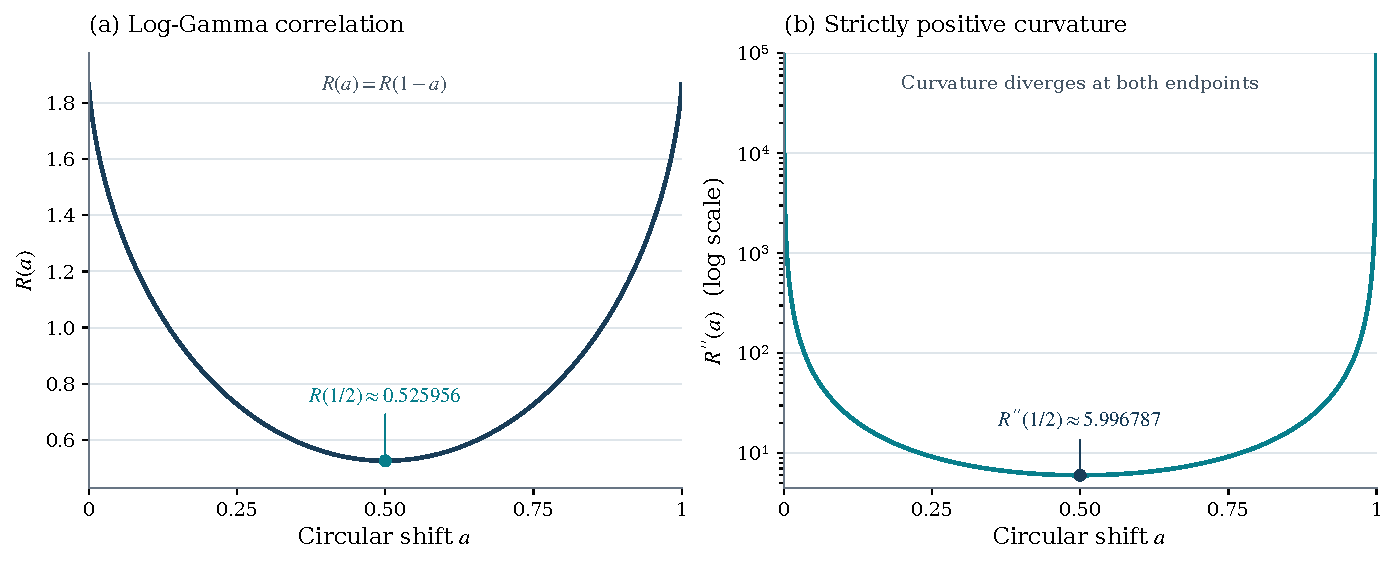
\includegraphics[width=\textwidth]{figures/loggamma_correlation.pdf}
 \caption{The ordinary circular log-Gamma correlation and its curvature.
 The plot uses the convergent expansion \eqref{eq:cusp} and the series
 \eqref{eq:Rsecondseries}; the analytic statements and strict inequalities
 follow from the proofs, not from the plot. Both minima occur at $a=1/2$.}
 \label{fig:correlation}
\end{figure}

\subsection{Recovery of a known Dilcher series}
\label{sec:dilcher}

Setting $R'(1/2)=0$ in the differentiated expansion gives
\begin{equation}\label{eq:Dilcher}
 \gamma_1+\frac12\log^22
       =\sum_{m\ge1}\frac{H_{2m}\zeta(2m+1)+\zeta'(2m+1)}{(2m+1)4^m}.
\end{equation}
Every summand is positive. The tail after $m=M\ge0$ is less than
$\zeta(3)/(3\cdot4^M)$, by $H_{2m}<2m+1$.
In particular $\gamma_1>-(\log2)^2/2$ follows without a decimal
evaluation.

This identity is not claimed as new. Brede \cite[printed p.~16]{Brede}
attributes the equivalent formula
\begin{equation}\label{eq:Dilcheroriginal}
 \gamma_1=-\frac12\log^2(3/2)
 +\sum_{m\ge1}
 \frac{H_{2m}(\zeta(2m+1)-1)+\zeta'(2m+1)}{(2m+1)4^m}
\end{equation}
to Dilcher \cite{Dilcher}. Equivalence follows from
\[
 \sum_{m\ge1}\frac{H_{2m}}{(2m+1)4^m}
       =\frac12\bigl(\log^22-\log^2(3/2)\bigr).
\]
For a direct verification, take the even part of
$\sum_{n\ge0}H_nx^n=-\log(1-x)/(1-x)$, integrate from $0$ to $1/2$,
and divide by $1/2$. The source chain is explicit because the present
audit verified the displayed identity in Brede's accessible dissertation
and the primary Dilcher article's bibliographic record, without access
to the full Dilcher text.

\section{All negative-integer jets and Stieltjes antiderivatives}
\label{sec:alljets}

The log-Gamma case is the first member of a larger exact regularity
theorem. For integers $p,r\ge0$ set
\begin{equation}\label{eq:Zpr}
 Z_{p,r}(x)=\zeta^{(r)}(-p,x),\qquad
 R_{p,r}(a)=\int_0^1 Z_{p,r}(x)Z_{p,r}(\{x+a\})\dd x.
\end{equation}
All these functions are in $L^2(0,1)$ and have mean zero. Their
correlations are real and even. Write $H_0^{(j)}=0$ and define the monic
polynomial
\begin{equation}\label{eq:jetpolynomial}
 P_{p,r}(z)=r![u^r]\exp\left(zu+
                \sum_{j\ge2}\frac{\zeta(j)-H_p^{(j)}}j u^j\right).
\end{equation}
Only terms through degree $r$ in this exponential contribute. Put
\begin{equation}\label{eq:Qjetpolynomial}
 Q_{p,r}(y)=P_{p,r}(y+A-H_p+\pi\iu/2)
           P_{p,r}(y+A-H_p-\pi\iu/2).
\end{equation}
Its coefficients are real and its degree is $2r$.

\begin{theorem}[Complete collision polynomial for every jet]
\label{thm:alljets}
Define
\begin{equation}\label{eq:Eprk}
 E_{p,r,k}=\frac{2(p!)^2}{(2\pi)^{2p+2}}
       \frac{(-1)^k(2\pi)^{2k}}{(2k)!}
       \left.Q_{p,r}(-\partial_w)\zeta(w-2k)\right|_{w=2p+2},
       \qquad k\ge0,
\end{equation}
and the holomorphic beta germ
\begin{equation}\label{eq:Kp}
 K_p(u,v)=\frac{(-1)^{p+1}}2
 \mathrm B(p+1-u,p+1-v)
 \frac{\cos(\pi(u-v)/2)}{\cos(\pi(u+v)/2)}.
\end{equation}
Here $\mathrm B(x,y)=\Gamma(x)\Gamma(y)/\Gamma(x+y)$.
Then for every $0<a<1$,
\begin{equation}\label{eq:alljetsexact}
 R_{p,r}(a)=\sum_{k\ge0}E_{p,r,k}a^{2k}
 +a^{2p+1}(r!)^2[u^rv^r]
                \left(K_p(u,v)e^{-(u+v)\log a}\right).
\end{equation}
The series converges normally for $|a|<1$. The second term is
$a^{2p+1}$ times a polynomial of degree $2r$ in $\log a$, all of whose
coefficients are determined by the finite germ in \eqref{eq:Kp}.
\end{theorem}
\begin{proof}
Differentiate the Hurwitz Fourier coefficient at $s=-p$. Since
\[
 \log\frac{\Gamma(p+1-u)}{p!}
  =(\gamma-H_p)u+
                \sum_{j\ge2}\frac{\zeta(j)-H_p^{(j)}}j u^j,
\]
the positive Fourier coefficients are
\begin{equation}\label{eq:jetFourier}
 \widehat Z_{p,r}(n)=
 \frac{p!e^{-\pi\iu(p+1)/2}}{(2\pi n)^{p+1}}
      P_{p,r}(\log n+A-H_p+\pi\iu/2),\qquad n\ge1.
\end{equation}
Their integrals and parameter derivatives are justified on a sufficiently
small spectral disk by majorants
$C[1+x^{p-\epsilon}(1+|\log x|^r)]$, with fixed $0<\epsilon<1/2$.
These include the bounded shifted Hurwitz remainder and belong to $L^2$;
the resulting Fourier families also converge in $L^2$.
Squaring their absolute values shows
\begin{equation}\label{eq:jetoperator}
 R_{p,r}(a)=\left.\frac{2(p!)^2}{(2\pi)^{2p+2}}
           Q_{p,r}(-\partial_w)\mathcal L_w(a)\right|_{w=2p+2}.
\end{equation}
The even analytic terms in \eqref{eq:symmetricjonquiere} give precisely
\eqref{eq:Eprk}. None of their zeta arguments is $1$ at this even
evaluation order, so there is no unpaired pole.

To compute the nonanalytic term without expanding many derivatives,
symmetrize \eqref{eq:hurwitzplus} in $s,t$ before taking equal-order
jets. This gives
\[
 \frac{\calK_+(s,t;a)+\calK_+(t,s;a)}2
 =2\Gamma(1-s)\Gamma(1-t)(2\pi)^{s+t-2}
       \cos\frac{\pi(s-t)}2\,\mathcal L_{2-s-t}(a).
\]
Its fractional-power coefficient is
\[
 \frac{\Gamma(1-s)\Gamma(1-t)\Gamma(s+t-1)}{2\pi}
                      (\sin\pi s+\sin\pi t).
\]
Substitute $s=-p+u,t=-p+v$. Euler reflection converts this coefficient
to $K_p(u,v)$; the zero in the sum of sines cancels the apparent
gamma pole. The power is $a^{2p+1-u-v}$.
Taking $\partial_u^r\partial_v^r$ proves the collision term in
\eqref{eq:alljetsexact}. Normal convergence of the local polylogarithm
expansion on compact parameter disks justifies every differentiation and
the stated convergence.
\end{proof}

For the first jet $r=1$, the whole collision polynomial simplifies to
\begin{align}\label{eq:firstjetcusp}
 R_{p,1}(a)={}&\sum_{k\ge0}E_{p,1,k}a^{2k}
 +\frac{(-1)^{p+1}(p!)^2a^{2p+1}}{2(2p+1)!}\notag\\
 &\times\left[(\log a-H_{2p+1}+H_p)^2
                       +H_{2p+1}^{(2)}+\frac{\pi^2}{3}\right].
\end{align}
To check the coefficient explicitly, the first logarithmic derivative of
$K_p$ at zero is $H_{2p+1}-H_p$, and its mixed logarithmic derivative is
$H_{2p+1}^{(2)}+\pi^2/3$. With $p=0$, formula
\eqref{eq:firstjetcusp} recovers the nonanalytic part of
Theorem~\ref{thm:cusp}.

For a higher example, $p=0,r=2$, let $T=1-\log a$. The complete
collision contribution is
\begin{equation}\label{eq:secondjetcusp}
 -\frac a2\left[T^4+(6+8\zeta(2))T^2+8(1-\zeta(3))T
                          +9+8\zeta(2)+14\zeta(4)\right].
\end{equation}
It follows by extracting $[u^2v^2]$ in the holomorphic germ, so its
constants are exact and do not rely on a numerical fit.

\begin{corollary}[Sharp regularity]\label{cor:jetregularity}
On $\T$, for $p,r\ge0$,
\begin{equation}\label{eq:jetregularity}
 R_{p,r}\in C^{2p},\qquad R_{p,r}\notin C^{2p+1}.
\end{equation}
For $r\ge1$ one has $R_{p,r}\in C^{2p,\alpha}$ for every $0<\alpha<1$,
but $R_{p,r}\notin C^{2p,1}$. For $r=0$ it belongs to $C^{2p,1}$ and
its next derivative has a jump at the seam. The exact Sobolev thresholds
are
\begin{equation}\label{eq:sobolev}
 Z_{p,r}\in H^q(\T)\ \Longleftrightarrow\ q<p+\tfrac12,
 \qquad
 R_{p,r}\in H^q(\T)\ \Longleftrightarrow\ q<2p+\tfrac32.
\end{equation}
\end{corollary}
\begin{proof}
Since $P_{p,r}$ is monic, \eqref{eq:jetFourier} has magnitude
asymptotic to
$p!n^{-p-1}(\log n)^r/(2\pi)^{p+1}$.
The correlation coefficients are its squared magnitudes. The weighted
square-sum definition of $H^q$ proves \eqref{eq:sobolev}, including
divergence at both threshold exponents.

The leading coefficient of the logarithmic collision polynomial is
\begin{equation}\label{eq:universalcollision}
 K_p(0,0)=\frac{(-1)^{p+1}(p!)^2}{2(2p+1)!}.
\end{equation}
Indeed the factor $(r!)^2[u^rv^r]e^{-(u+v)\log a}$ has leading term
$\log^{2r}a$. The analytic even series and all its relevant derivatives
converge through the seam, whereas the collision term has a continuous
$2p$th derivative and
\begin{equation}\label{eq:jetseam}
 R_{p,r}^{(2p)}(a)-R_{p,r}^{(2p)}(0)
 \sim\frac{(-1)^{p+1}(p!)^2}{2}|a|\log^{2r}|a|.
\end{equation}
For $r=0$ the logarithmic factor means $1$. This proves the failure of
the next derivative and, when $r\ge1$, the failure of Lipschitz
continuity of the $2p$th derivative. The elementary bound
$h(1+|\log h|^{2r})=O(h^\alpha)$ for $\alpha<1$, applied to the local
collision polynomial, proves the asserted H\"older regularity. Away
from the seam everything is real analytic.
\end{proof}

\subsection{Application to the normalized Stieltjes primitive}

Use the manuscript's normalization
\begin{equation}\label{eq:Stieltjesprimitive}
 \mathcal A_n(x)=\frac{(-1)^{n+1}}{n+1}
       \bigl(\zeta^{(n+1)}(0,x)-\zeta^{(n+1)}(0)\bigr).
\end{equation}
Then $\mathcal A_n(1)=0$ and $\mathcal A_n'(x)=\gamma_n(x)$.
The latter follows by taking the coefficient of $s^{n+1}$ in
$\partial_x\zeta(s,x)=-s\zeta(s+1,x)$; it is one of the existing
antiderivative identities, included here to fix the normalization.
After subtracting its mean, $\mathcal A_n$ is
$(-1)^{n+1}Z_{0,n+1}/(n+1)$. Its circular covariance $V_n$ therefore
has the exact representation $V_n=R_{0,n+1}/(n+1)^2$ and
\begin{equation}\label{eq:primitivecusp}
 V_n(0)-V_n(a)\sim\frac{a}{2(n+1)^2}\log^{2n+2}(1/a).
\end{equation}
The full logarithmic polynomial is given by Theorem~\ref{thm:alljets},
not only its leading coefficient. In particular every one of these
primitive covariances is H\"older of every exponent below one and fails
to be Lipschitz. This extends the antiderivative formulas to sharp
analytic information about their translated products.

The balanced negative-polygamma combination
\[
 \Psi_{p+1}(x)=\frac{\zeta'(-p,x)+H_p\zeta(-p,x)}{p!}
\]
has the similarly explicit collision contribution
\begin{equation}\label{eq:balancedcusp}
 \frac{(-1)^{p+1}a^{2p+1}}{2(2p+1)!}
       \left[(\log a-H_{2p+1})^2
                         +H_{2p+1}^{(2)}+\frac{\pi^2}{3}\right].
\end{equation}
Its analytic coefficients follow from \eqref{eq:Eprk} by replacing the
first-jet polynomial $z$ with $z+H_p$ and dividing by $(p!)^2$.

\section{Positive moments in the Stieltjes derivative tower}
\label{sec:hankel}

The derivative identities admit a complementary nonlinear consequence.
It comes from a positive measure, rather than a numerical search for
linear relations. Let $a>0$, $k\ge1$, and $p=k+1$. Define
\begin{equation}\label{eq:fn}
 f_n=\frac{(-1)^k}{k!}\gamma_n^{(k)}(a),\qquad n\ge0.
\end{equation}
The parameter-derivative identity yields
\begin{equation}\label{eq:fgenerator}
 \sum_{n\ge0}f_n\frac{z^n}{n!}
     =\prod_{j=1}^k\left(1-\frac zj\right)\zeta(p-z,a).
\end{equation}
The right side is entire in $z$: the polynomial cancels the sole
Hurwitz pole, at $z=k$. In particular, these are actual globally
convergent Taylor series, not merely formal expansions.

Let $h_r=h_r(1,1/2,\ldots,1/k)$ be the complete homogeneous symmetric
polynomial, with $h_0=1$, so that
\[
 \prod_{j=1}^k(1-z/j)^{-1}=\sum_{r\ge0}h_r z^r
 \quad\hbox{near }z=0.
\]
The compensated coefficients are
\begin{equation}\label{eq:Mn}
 M_n=\sum_{r=0}^n\frac{n!}{(n-r)!}h_r f_{n-r}
       =(-1)^n\zeta^{(n)}(p,a)
       =\sum_{j\ge0}\frac{\log^n(a+j)}{(a+j)^p}.
\end{equation}
The compensated generating function $\zeta(p-z,a)$ does have a pole
at $z=k$; it should be distinguished from the entire function in
\eqref{eq:fgenerator}.

\begin{theorem}[Strict Hankel positivity and an exact determinant]
\label{thm:hankel}
For every $a>0$, real $p>1$, and integer $d\ge1$, define
$M_n=(-1)^n\zeta^{(n)}(p,a)$. Then
\begin{align}\label{eq:Hankelsum}
 D_d(p,a):=\det[M_{i+j}]_{0\le i,j<d}
 =\sum_{0\le j_1<\cdots<j_d}
 \prod_{v=1}^d(a+j_v)^{-p}
 \prod_{1\le u<v\le d}
        \log^2\left(\frac{a+j_v}{a+j_u}\right)>0.
\end{align}
Thus every finite Hankel moment matrix is strictly positive definite.
At integer $p=k+1$, \eqref{eq:Mn} expresses all these strict
inequalities as polynomial inequalities in Stieltjes parameter
derivatives.
\end{theorem}
\begin{proof}
The positive discrete measure
\[
 \mu_{p,a}=\sum_{j\ge0}(a+j)^{-p}\delta_{\log(a+j)}
\]
has finite moments of every order and exactly the moments $M_n$.
For a nonzero polynomial $q$,
$\int q(t)^2\dd\mu_{p,a}(t)>0$, because infinitely many distinct
support points cannot all be roots of $q$. This proves strict positive
definiteness. For the determinant identity, restrict the measure to
$0\le j\le N$. Its Gram matrix factors as the product of a monomial
evaluation matrix, the diagonal weights, and the transpose evaluation
matrix. The finite Cauchy--Binet identity gives the sum of the squared
Vandermonde minors displayed in \eqref{eq:Hankelsum}. Let $N\to\infty$.
The moments, hence determinants, converge absolutely; the positive
tuple sums increase to the same limit. This proves the identity and
strictness without a cancellation estimate.
\end{proof}

For $a\ge1$, this is a Stieltjes moment measure, supported on
$[0,\infty)$. When $0<a<1$, its first support point is negative, so
the correct general description is a Hamburger moment measure; odd
moments need not be positive. The Hankel conclusions hold in both cases.

\begin{corollary}[A strict nonlinear Stieltjes inequality]
\label{cor:StieltjesHankel}
For every $a>0$ and integer $k\ge1$,
\begin{align}\label{eq:Stieltjesineq}
 &\gamma_0^{(k)}(a)\gamma_2^{(k)}(a)
   -\bigl(\gamma_1^{(k)}(a)\bigr)^2
   +H_k^{(2)}\bigl(\gamma_0^{(k)}(a)\bigr)^2\notag\\
 &\hspace{18mm}>(k!)^2[a(a+1)]^{-k-1}\log^2(1+1/a)>0.
\end{align}
\end{corollary}
\begin{proof}
From \eqref{eq:Mn},
$M_0=f_0$, $M_1=f_1+H_kf_0$, and
$M_2=f_2+2H_kf_1+(H_k^2+H_k^{(2)})f_0$.
Thus $M_0M_2-M_1^2=f_0f_2-f_1^2+H_k^{(2)}f_0^2$.
In \eqref{eq:Hankelsum}, the pair $(j_1,j_2)=(0,1)$ contributes the
right side divided by $(k!)^2$, and all other pairs contribute
strictly positive terms. Multiplication by $(k!)^2$ proves the claim.
\end{proof}

The cancellation of $H_k$ at order two has an all-order explanation.
Translation of the moment coordinate by $-H_k$ preserves every Hankel
determinant: the binomial change of monomials is triangular with diagonal
one and acts by congruence on the Gram matrix. The translated generating
function, as an identity of germs at $z=0$ (and for $|z|<1$), is
\begin{equation}\label{eq:translatedmoments}
 e^{-H_kz}\zeta(p-z,a)
 =\exp\left(\sum_{j\ge2}\frac{H_k^{(j)}}j z^j\right)
                     \sum_{n\ge0}f_n\frac{z^n}{n!}.
\end{equation}
For example, with $h_j^*=H_k^{(j)}$, the strictly positive $d=3$
determinant is that of the matrix
\begin{equation}\label{eq:Hankel3}
 \begin{pmatrix}
 f_0&f_1&f_2+h_2^*f_0\\
 f_1&f_2+h_2^*f_0&f_3+3h_2^*f_1+2h_3^*f_0\\
 f_2+h_2^*f_0&f_3+3h_2^*f_1+2h_3^*f_0&
 f_4+6h_2^*f_2+8h_3^*f_1+(3(h_2^*)^2+6h_4^*)f_0
 \end{pmatrix}.
\end{equation}
Equation~\eqref{eq:translatedmoments} is usually more convenient than
expanding larger determinants by hand.

\subsection{A sharp asymptotic in derivative order}

Fix $a>0$ and $d\ge1$. Write
\begin{align}
 A_0&=\prod_{j=0}^{d-1}(a+j),&
 V_0&=\prod_{0\le i<j<d}\log^2\left(\frac{a+j}{a+i}\right),&
 T_0(p)&=A_0^{-p}V_0,\label{eq:A0V0}\\
 \rho_1&=\frac{a+d-1}{a+d},&
 C_1&=\prod_{j=0}^{d-2}
 \left[\frac{\log((a+d)/(a+j))}{\log((a+d-1)/(a+j))}\right]^2,&
 \rho_2&=\frac{a+d-1}{a+d+1}.
 \label{eq:rho}
\end{align}
All empty products, including those for $d=1$, equal one.

\begin{theorem}[Two leading exponential terms and a rigorous remainder]
\label{thm:Hankelasymptotic}
As $p\to+\infty$, with $a,d$ fixed,
\begin{equation}\label{eq:Hankelasymp}
 \frac{D_d(p,a)}{T_0(p)}
                  =1+C_1\rho_1^p+O(\rho_2^p).
\end{equation}
More precisely, for $p\ge p_0>1$,
\begin{equation}\label{eq:Hankelremainder}
 0\le\frac{D_d(p,a)}{T_0(p)}-1-C_1\rho_1^p
 \le E_d(p_0,a)\rho_2^{p-p_0},
\end{equation}
where the explicit positive constant is
\begin{equation}\label{eq:Ed}
 E_d(p_0,a)=\frac{D_d(p_0,a)}{T_0(p_0)}-1-C_1\rho_1^{p_0}>0.
\end{equation}
\end{theorem}
\begin{proof}
The smallest tuple product in \eqref{eq:Hankelsum} is uniquely that of
$(0,\ldots,d-1)$, contributing $T_0(p)$. The next tuple is
$(0,\ldots,d-2,d)$, whose normalized term is $C_1\rho_1^p$.
Among the remaining tuples, changing only the last coordinate gives
the smallest product at $(0,\ldots,d-2,d+1)$, with base $\rho_2$.
For $d\ge2$, changing an earlier coordinate forces the last two to be
at least $d-1,d$; its product ratio relative to the first tuple is at
least $(a+d)/(a+d-2)$. This is strictly greater than
$(a+d+1)/(a+d-1)$, the ratio for the third tuple. The assertion for
$d=1$ is immediate. Hence every omitted normalized base $b$ satisfies
$0<b\le\rho_2<1$.

Write its positive normalized Vandermonde weight as $c$. For
$p\ge p_0$, one has $cb^p\le cb^{p_0}\rho_2^{p-p_0}$.
Sum this inequality over the omitted tuples. Their sum at $p_0$ is
exactly \eqref{eq:Ed}, proving \eqref{eq:Hankelremainder} and then
\eqref{eq:Hankelasymp}. Strict positivity of $E_d$ follows from the
third tuple itself.
\end{proof}

For the Stieltjes derivative tower take $p=k+1$ and, for example,
$p_0=2$. This is a rigorous large-derivative-order asymptotic for the
normalized nonlinear combinations in \eqref{eq:Mn}. It is not stated
uniformly when $a$ or $d$ grows. Higher exponential terms follow from
the exact positive tuple sum; equal products from different later tuples
must be grouped if one orders the expansion by distinct bases.

An elementary consequence of the entire generating function, separate
from positivity, is
\begin{equation}\label{eq:derivativeexpsums}
 \sum_{n\ge0}\gamma_n^{(k)}(a)\frac{j^n}{n!}
 =\begin{cases}
       0,&j=1,\ldots,k-1,\\
       -(k-1)!,&j=k.
   \end{cases}
\end{equation}
For $j<k$, a polynomial zero in \eqref{eq:fgenerator} multiplies a
finite Hurwitz value. For $j=k$, cancel the simple pole before taking
the limit; the residue gives $-(k-1)!$. The convergence here is actual
Taylor convergence of an entire function.

\section{Proposed corrections to the current manuscript}
\label{sec:corrections}

The two proposed edits below are limited to
\sourcepath{Analysis/Polylogarithms/docs/manuscript/chapters/07-integration.tex}
at the pinned snapshot. The package includes a minimal unified patch,
with context and source hash, so the changes can be reviewed separately
from adding the present article. Neither edit changes the coefficients
of an existing special-function identity.

\subsection{The Hurwitz ladder needs an explicit convergence domain}

At the label \texttt{integral:res:hurwitzladder}, the manuscript prints
\begin{equation}\label{eq:Hurwitzladder}
 \log\Gamma(z)=\left(z-\tfrac12\right)\log z-z+\frac12\log(2\pi)
 +\frac12\sum_{n\ge2}\frac{n-1}{n(n+1)}\zeta(n,z+1).
\end{equation}
The formula is correct on $\Rea z>0$, with the analytic branch of
$\log\Gamma$ normalized on the positive real axis and the principal
$\log z$. That sufficient domain should be stated. The unqualified
series is not valid at all regular gamma arguments: at $z=-1/2$,
$\zeta(n,1/2)=(2^n-1)\zeta(n)$, so its summands do not even tend to
zero. This is a convergence-domain omission, not a wrong-coefficient
claim.

\begin{proposition}[Convergence and an explicit ladder remainder]
\label{prop:ladder}
Equation~\eqref{eq:Hurwitzladder} holds with locally uniform absolute
convergence on $\Rea z>0$. If $N\ge2$ and $\Rea z\ge\sigma>0$, the
tail after $n=N$ satisfies
\begin{equation}\label{eq:laddertail}
 |\mathrm{tail}_N(z)|
 \le\frac{\zeta(N,\sigma+1)}{2(N+1)\sigma}
 \le\frac{(\sigma+1)^{-N}+(\sigma+1)^{1-N}/(N-1)}{2(N+1)\sigma}.
\end{equation}
\end{proposition}
\begin{proof}
For real $w>1$, elementary summation of the power series gives
\begin{equation}\label{eq:ladderscalar}
 \frac12\sum_{n\ge2}\frac{n-1}{n(n+1)}w^{-n}
                =(w-\tfrac12)\log\frac{w}{w-1}-1.
\end{equation}
For instance, use
$(n-1)/(n(n+1))=-1/n+2/(n+1)$ and the logarithmic power series.
For real $z>0$, the positive terms permit interchange with
$\zeta(n,z+1)=\sum_{m\ge0}(z+m+1)^{-n}$.
Let
\[
 B(z)=\log\Gamma(z)-(z-\tfrac12)\log z+z-\tfrac12\log(2\pi).
\]
The gamma recurrence gives
$B(z)-B(z+1)=(z+1/2)\log((z+1)/z)-1$.
Thus the sum of \eqref{eq:ladderscalar} over $w=z+m+1$,
$0\le m<M$, equals $B(z)-B(z+M)$. Stirling's formula implies
$B(z+M)\to0$, proving \eqref{eq:Hurwitzladder} on the positive axis.

For $\Rea z\ge\sigma>0$ and $n>N$,
$(n-1)/(n(n+1))\le1/(N+1)$ and
$|z+m+1|^{-n}\le(\sigma+m+1)^{-n}$. Summing the resulting geometric
series gives
\[
 |\mathrm{tail}_N(z)|\le\frac1{2(N+1)}
      \sum_{m\ge0}\frac{(\sigma+m+1)^{-N}}{\sigma+m}
 \le\frac{\zeta(N,\sigma+1)}{2(N+1)\sigma}.
\]
The elementary integral bound for a decreasing power series yields the
second inequality in \eqref{eq:laddertail}. These estimates prove local
uniform absolute convergence, so the identity theorem extends the
positive-axis formula to the right half-plane.
\end{proof}

The proposed source edit inserts the domain and branch convention before
the displayed ladder and a brief convergence statement afterward.
The detailed proof and reusable error bound remain in this article.

\subsection{Integer-relation searches do not require an independence theorem}

At \texttt{integral:neg:psim2}, the sentence requiring the basis atoms
to be $\Q$-independent is too strong. The observed issue is that known
dependencies among the background coordinates can make a one-relation
search return a relation whose target coefficient is zero. Removing
known dependencies is good practice; proving actual arithmetic
independence of the remaining constants is not a prerequisite for a
valid search.

The proposed replacement is:
\begin{quote}
Remove known dependencies from the background coordinates, or retain
them explicitly and search modulo their known relation space. A returned
relation must have a nonzero target coefficient to evaluate the target.
No unproved arithmetic-independence assumption is needed.
\end{quote}
This is a correction to the methodological wording. It does not change
the recorded failed experiment or rehabilitate its rejected candidate.
The current discovery chapter already distinguishes formal coordinates
from arithmetic independence, so the edit also makes the explanations
consistent across the manuscript.

\section{Further research questions}
\label{sec:questions}

The following questions separate tractable extensions from statements
that need substantially new arguments. They are proposals for further
work; none is used as an assumption in the proofs above.

\begin{enumerate}[leftmargin=*,label=\textbf{\arabic*.},itemsep=7pt]
\item \textbf{Products at three or more independent shifts.}
Determine an explicit generating function for
\[
 \FP\int_0^1\prod_{j=1}^r\gamma_{n_j}(\{x+a_j\})\dd x,
 \qquad r\ge3,
\]
first with distinct shifts and then as selected shifts coalesce.
These are simultaneous pointwise products, not iterated convolutions,
which are already controlled by Theorem~\ref{thm:algebra}.
The Fourier constraint now leaves several summation indices, suggesting
multiple polylogarithms and Tornheim-type derivatives. A useful first
goal is a complete three-factor subtraction formula with every local
counterterm specified.

\item \textbf{Uniform collision asymptotics with growing jet order.}
Theorem~\ref{thm:alljets} fixes $p,r$, and the finite-part theorem fixes
$n,m$. Obtain estimates uniform when an index grows while $a\to0$.
The competition between factorial coefficient growth, gamma singularities
in the generating variables, and powers of $\log a$ is absent from the
fixed-index arguments. An explicit transition scaling and error bound
would make the identities useful at high weight.

\item \textbf{Sign and extremum classification for higher jet correlations.}
The full positivity of the even derivatives of $R$ is stronger than
positive definiteness of an autocorrelation kernel. Decide which
$R_{p,r}$, or which derivatives and balanced combinations of them,
retain an analogous sign pattern. For $p>0$, the Bernoulli cases already
have a different pattern, so the log-Gamma conclusion should not be
extrapolated without proof. The explicit coefficients in
\eqref{eq:Eprk} give a precise starting point for counterexamples or
classification theorems.

\item \textbf{Optimal inequalities for higher Stieltjes reflection sums.}
The sharp midpoint inequality \eqref{eq:reflectionineq} treats index one.
For $n\ge2$, determine the extrema and sign changes of
$\gamma_n(a)+\gamma_n(1-a)$ and of the universal lower-index corrections
appearing in $F^+_{n,m}$. Formulate the problem at the level of complete
correlation derivatives so that any endpoint singular terms are retained.

\item \textbf{Rational shifts, characters, and exact relation spaces.}
Combine Theorem~\ref{thm:triangular} with the manuscript's character and
conductor descent. At a fixed conductor and total index, compute the
formal span of the resulting bilinear identities and its exact
relations. Separate this finite symbolic quotient from the much harder
question of arithmetic independence of the evaluated constants.
Useful deliverables would be small, replayable rational certificates,
not only reduced decimal expressions.

\item \textbf{Normalization under rescaling and nonlinear changes of variable.}
Theorem~\ref{thm:derivative} fixes one coordinate and scale. Classify how
the finite parts and their Dirac derivatives transform when the period
or local coordinate changes. Determine which combinations of zero mean,
reflection symmetry, differentiation, and the Hurwitz semigroup can be
preserved simultaneously. This would give a principled way to compare
different regularization conventions used in symbolic integrations.

\item \textbf{Large Hankel dimension and joint parameter limits.}
Theorem~\ref{thm:Hankelasymptotic} fixes $a,d$. Find a uniform asymptotic
when $d$ grows with $p$, or when $a$ also varies. The exact positive
Vandermonde sum provides explicit candidates for the dominant tuples,
but control of their number and near-equal products is required.
Bounds for the smallest eigenvalue would turn determinant positivity
into quantitative stability estimates for the derivative tower.

\item \textbf{Certified high-order evaluation.}
Turn the coefficient algorithms and Cauchy order-differentiation checks
into interval enclosures. For a finite-radius contour, derive an explicit
trapezoidal aliasing bound from a larger analytic annulus and include
the evaluation errors at every node. Combine it with
\eqref{eq:cusptail} and the finite-part endpoint subtractions. This would
give certified numerical values without mistaking working precision for
an error certificate.

\item \textbf{The remaining mixed Gaussian candidates.}
The frozen $S_6$ relation and the new $S_8$ vector in
\texttt{s8new:conj:S8} remain genuine targets. Seek an exact convergent
word or shuffle certificate, building on the already proved $S_4$
transformation, or a rigorous nonzero residual. An interval containing
zero, however narrow, proves proximity only. The earlier rejected
$S_8$ vector must remain distinct from the new candidate.
The present convolution identities supply additional analytic
representations but do not provide those missing certificates.

\item \textbf{A precise reduction question for higher log-Gamma moments.}
The manuscript already has a Tornheim representation for the cubic
moment. Fix an explicit candidate algebra of single zeta and Dirichlet
$L$ derivatives and ask whether a reduction into it can be proved.
Shifted three-point correlations may expose useful functional equations
before taking the coincident-shift limit. Failure of a chosen finite
relation search would not establish irreducibility in that algebra.
\end{enumerate}

\section{Verification, reproducibility, and integration status}
\label{sec:verification}

The proofs establish the identities. Computations serve three narrower
purposes: they check finite symbolic expansions, compare independent
analytic representations numerically, and make the proposed source
edits reproducible. They are not used to infer an infinite identity from
a small residual.

\subsection{Exact algebra and independent numerical checks}

The file \sourcepath{verification/exact_coefficients.py} expands the
gamma germs in a rational polynomial ring with formal symbols for zeta
values and Stieltjes functions. It checks 60 exact assertions and exports
15 coefficient pairs, covering all $n+m\le4$ in both orientations.
No floating-point arithmetic or integer-relation search enters those
calculations. The companion
\sourcepath{verification/exact_jet_polynomials.py} checks the displayed
jet collision polynomials and their logarithmic derivatives symbolically.
These finite checks complement, rather than replace, the every-index
analytic proofs.

The numerical scripts use independent left and right sides where
practical. In particular, the finite-part integrals use ordinary real
quadrature after explicit local subtraction. The following values are
representative; all digits and settings are recorded in the JSON files.
\begin{center}
\small
\begin{tabular}{@{}lll@{}}
\toprule
Quantity & Value, rounded & Typical absolute discrepancy\\
\midrule
$F^+_{0,0}(1/2)$ & $-5.99678749530633590836$ & below $10^{-53}$\\
$F^-_{0,0}(1/2)$ & $-1.06198529476165659894$ & below $10^{-53}$\\
$F^+_{1,0}(\sqrt2-1)$ & $6.90546420565063770565$ & below $10^{-41}$\\
$F^-_{1,0}(\sqrt2-1)$ & $-2.43190584182042316367$ & below $10^{-41}$\\
$R(0)$ & $1.86631708379356208099$ & below $10^{-45}$\\
$R(1/2)$ & $0.52595583980330838858$ & below $10^{-45}$\\
\bottomrule
\end{tabular}
\end{center}
The finite-part files contain eleven zeroth-order checks at 55-digit
working precision and four mixed-index checks at 45 digits. The ordinary
correlation file contains sixteen checks at 48 digits, including real
parameters with $\Rea(s+t)>1$, a complex critical-order example, and
direct log-Gamma quadrature. This specifically tests the separated
singularity domain in Theorem~\ref{thm:classical}.

The raw derivative finite-part check uses \eqref{eq:k1cutoff} at
$a=1/2$ and $a=0.37$, with cutoffs down to $10^{-18}$ and 65 working
digits. Its unextrapolated discrepancy is of order $\epsilon$, as
expected. A Taylor expansion of the two omitted endpoint intervals gives
the first error coefficient
\[
 C(a)=\gamma\psi'(a)-\tfrac32\psi''(a)-\zeta(2)\psi(a).
\]
Subtracting $C(a)\epsilon$ leaves discrepancies below $1.2\cdot10^{-34}$
in the two final rows. These smaller errors reflect explicit cutoff
acceleration, not an interval proof of the integral value.

The Hankel/ladder file uses 80-digit arithmetic. It checks compensated
Stieltjes derivatives through index four for three parameter choices,
strict $d=2,3$ determinant bounds, finite Cauchy--Binet sums, twenty
tuple-order cases, thirty asymptotic remainder bounds, and six real or
complex Hurwitz-ladder examples. All use the domains and normalizations
stated in the theorems.

\subsection{A numerical implementation issue found during verification}

In the installed \texttt{mpmath 1.3.0}, applying the default infinitesimal
\texttt{mp.diff} directly to a boundary polylogarithm at an integer
order can lose accuracy in a precision-dependent way. One log-Gamma
check at 48 working digits had a discrepancy about $4.5\cdot10^{-13}$,
while finite-radius Cauchy differentiation agreed with independent real
quadrature to about $10^{-49}$. A similar problem occurred in an
order-zero second derivative at a different working precision. These
observations concern that evaluation path; they do not refute the
polylogarithm identities.

The final checks therefore use the Cauchy coefficient formula
\begin{equation}\label{eq:Cauchydiagnostic}
 f^{(r)}(w_0)\approx
 \frac{r!}{N\rho^r}\sum_{j=0}^{N-1}
 f(w_0+\rho e^{\iu\theta_j})e^{-\iu r\theta_j},
 \qquad\theta_j=\frac{2\pi(j+1/2)}N,
\end{equation}
with $\rho=1/8$ and $N=64$, instead of the vulnerable path. The full
finite-contour remainder is not interval-certified in these scripts.
Its agreement with separately subtracted real quadrature is numerical
evidence, clearly labeled as such in the outputs. The direct
\texttt{mp.diff} comparison is retained only as a diagnostic of the
implementation issue, not as a theorem-check acceptance test.

\subsection{Delivered sources and proposed integration}

The archive contains the complete standalone \TeX\ source, compiled
PDF, the correlation figure in PDF and PNG, runnable Python scripts,
JSON results, a build recipe, source provenance, and the minimal
correction patch. The source manifest records the pinned Git commit and
hashes of the repository files consulted. No repository change is
implied by delivery of the patch.

For integration, the most natural route is a bilinear-calculus section
after the existing Stieltjes derivative and antiderivative material,
with a cross-reference from the log-Gamma moment chapter. The Hankel
section can also stand as a separate derivative-tower continuation.
The standalone labels should receive a common prefix when merged with
the main manuscript; the accompanying integration note gives the
specific dependency order. Classical formulas should retain their
attribution, the finite-part convention must accompany the displayed
integrals, and the distributional contact terms must accompany global
convolution identities.

\appendix
\section{Unequal jets and resonant collision cancellation}
\label{app:resonance}

For completeness, the shifted master kernel gives an explicit route to
unequal spectral orders as well. Put $\sigma=s+t$ and suppose initially
$\Rea s,\Rea t<1$ and $\sigma\notin\{1,0,-1,\ldots\}$.
The unsymmetrized local polylogarithm expansion gives the convergent
identity, for $0<a<1$,
\begin{align}\label{eq:generalcollision}
 \calK_+(s,t;a)={}&
 \frac{\Gamma(1-s)\Gamma(s+t-1)}{\Gamma(t)}a^{1-s-t}\notag\\
 &+2\Gamma(1-s)\Gamma(1-t)(2\pi)^{s+t-2}
 \sum_{j\ge0}\frac{\zeta(2-s-t-j)}{j!}
       \cos\frac{\pi(s-t-j)}2\,(2\pi a)^j.
\end{align}
The coefficient of the fractional power is
$\mathrm B(1-s,s+t-1)$ by analytic continuation. It also follows
independently from the local scaling integral of
$x^{-s}(x+a)^{-t}$ where that integral converges.

At $\sigma=1-M$ with $M\ge0$, the fractional term and the $j=M$
term in the sum can have poles separately. They must be combined before
taking the limit or differentiating. Here is an explicit holomorphic
prescription for all unequal negative-integer jets. For integers $p,q\ge0$,
put $s=-p+u$, $t=-q+v$, $M=p+q+1$, $w=u+v$, and let
\[
 b(u,v)=w\,\mathrm B(1-s,s+t-1),
\]
while $d(u,v)$ is $w$ times the coefficient of $a^M$ in the analytic
series in \eqref{eq:generalcollision}. Both are holomorphic near zero.
Since the full kernel is holomorphic, their residues cancel:
$b(u,-u)+d(u,-u)=0$. The resonant pair equals
\begin{equation}\label{eq:resonantpair}
 a^M\left[
 b(u,v)\frac{e^{-w\log a}-1}{w}
               +\frac{b(u,v)+d(u,v)}w\right].
\end{equation}
Both quotients are holomorphic. Taylor extraction now gives unequal
jet orders with no differentiation of an uncancelled pole. The
symmetric equal-order theorem in Section~\ref{sec:alljets} is the
particularly simple case where the cancellation is already absorbed
into the beta/cosine germ.

If also $\Rea(s+t)<1$, the singularities may coincide in the ordinary
integral and
\begin{align}\label{eq:coincidentclassical}
 \calK_+(s,t;0)
 &=\int_0^1\zeta(s,x)\zeta(t,x)\dd x\notag\\
 &=2\Gamma(1-s)\Gamma(1-t)(2\pi)^{s+t-2}
       \cos\frac{\pi(s-t)}2\,\zeta(2-s-t).
\end{align}
This additional condition controls the generic product singularity
$x^{-s-t}$; it is not needed at a fixed nonzero shift. At the other
seam, $a\to1$, interchange $s$ and $t$. These distinctions explain why
an unshifted product formula cannot simply be used to infer a shifted
integrability restriction.

\begin{thebibliography}{99}
\bibitem{ProveIt}
V.~Reshetnikov, \emph{ProveIt}, polylogarithm manuscript, editorial
ledger, and incoming archive register, snapshot
\texttt{570b0567f311cf1890865065896be2665f469e4f}, 10 October 2026.
\url{https://github.com/VladimirReshetnikov/ProveIt/tree/570b0567f311cf1890865065896be2665f469e4f/Analysis/Polylogarithms/docs/manuscript}.
Incoming register:
\url{https://github.com/VladimirReshetnikov/ProveIt/tree/570b0567f311cf1890865065896be2665f469e4f/docs/incoming}.

\bibitem{DLMFHurwitz}
NIST Digital Library of Mathematical Functions, \S25.11,
\emph{Hurwitz Zeta Function}; in particular 25.11.3, 25.11.9,
25.11.12, and the parameter and spectral derivative formulas.
\url{https://dlmf.nist.gov/25.11}. Accessed 10 October 2026.

\bibitem{DLMFPolylog}
NIST Digital Library of Mathematical Functions, \S25.12,
\emph{Polylogarithms}; especially the local expansion 25.12.12.
\url{https://dlmf.nist.gov/25.12}. Accessed 10 October 2026.

\bibitem{DLMFZeta}
NIST Digital Library of Mathematical Functions, \S25.4,
\emph{Reflection Formulas}; especially 25.4.2.
\url{https://dlmf.nist.gov/25.4}. Accessed 10 October 2026.

\bibitem{EspinosaMoll}
O.~Espinosa and V.~H.~Moll, On some integrals involving the Hurwitz
zeta function: Part 1, \emph{The Ramanujan Journal} \textbf{6}
(2002), 159--188.
\url{https://www.math.tulane.edu/~vhm/papers_html/hurwitz1.pdf}.

\bibitem{Sun}
Z.-H.~Sun, On the properties of invariant functions,
\emph{Bulletin des Sciences Math\'ematiques} \textbf{189} (2023), 103347.
Primary preprint arXiv:2209.14625v1 (2022), Remark 3.2, printed p.~15.
\url{https://arxiv.org/pdf/2209.14625v1}.

\bibitem{ZhuHuKim}
H.~Zhu, S.~Hu, and M.-S.~Kim, On the properties of alternating invariant
functions, arXiv:2505.10985v1 (2025), Theorem 1.6.
\url{https://arxiv.org/html/2505.10985v1}.

\bibitem{GaySebbar}
R.~Gay and A.~Sebbar, Pseudo-differential operators on the circle,
Bernoulli polynomials, \emph{Quantum Studies: Mathematics and
Foundations} \textbf{11} (2024), 1--25.
\url{https://doi.org/10.1007/s40509-024-00316-9}.

\bibitem{Dilcher}
K.~Dilcher, On generalized gamma functions related to the Laurent
coefficients of the Riemann zeta function,
\emph{Aequationes Mathematicae} \textbf{48} (1994), 55--85.
\url{https://doi.org/10.1007/BF01837979}.
The bibliographic record was consulted; the exact series attribution
used here is verified through \cite[printed p.~16]{Brede}.

\bibitem{Brede}
M.~Brede, \emph{Eine Reihenentwicklung der vervollst\"andigten und
erg\"anzten Riemannschen Zetafunktion und Verwandtes}, doctoral
dissertation, Universit\"at Gesamthochschule Kassel, 2001;
printed p.~16 for the series attributed to Dilcher.
\url{https://www.mathematik.uni-kassel.de/~koepf/Diplome/brede.pdf}.
\end{thebibliography}
\end{document}
